% Options for packages loaded elsewhere
\PassOptionsToPackage{unicode}{hyperref}
\PassOptionsToPackage{hyphens}{url}
\PassOptionsToPackage{dvipsnames,svgnames,x11names}{xcolor}
%
\documentclass[
  letterpaper,
  DIV=11,
  numbers=noendperiod]{scrreprt}

\usepackage{amsmath,amssymb}
\usepackage{lmodern}
\usepackage{iftex}
\ifPDFTeX
  \usepackage[T1]{fontenc}
  \usepackage[utf8]{inputenc}
  \usepackage{textcomp} % provide euro and other symbols
\else % if luatex or xetex
  \usepackage{unicode-math}
  \defaultfontfeatures{Scale=MatchLowercase}
  \defaultfontfeatures[\rmfamily]{Ligatures=TeX,Scale=1}
\fi
% Use upquote if available, for straight quotes in verbatim environments
\IfFileExists{upquote.sty}{\usepackage{upquote}}{}
\IfFileExists{microtype.sty}{% use microtype if available
  \usepackage[]{microtype}
  \UseMicrotypeSet[protrusion]{basicmath} % disable protrusion for tt fonts
}{}
\makeatletter
\@ifundefined{KOMAClassName}{% if non-KOMA class
  \IfFileExists{parskip.sty}{%
    \usepackage{parskip}
  }{% else
    \setlength{\parindent}{0pt}
    \setlength{\parskip}{6pt plus 2pt minus 1pt}}
}{% if KOMA class
  \KOMAoptions{parskip=half}}
\makeatother
\usepackage{xcolor}
\setlength{\emergencystretch}{3em} % prevent overfull lines
\setcounter{secnumdepth}{5}
% Make \paragraph and \subparagraph free-standing
\ifx\paragraph\undefined\else
  \let\oldparagraph\paragraph
  \renewcommand{\paragraph}[1]{\oldparagraph{#1}\mbox{}}
\fi
\ifx\subparagraph\undefined\else
  \let\oldsubparagraph\subparagraph
  \renewcommand{\subparagraph}[1]{\oldsubparagraph{#1}\mbox{}}
\fi

\usepackage{color}
\usepackage{fancyvrb}
\newcommand{\VerbBar}{|}
\newcommand{\VERB}{\Verb[commandchars=\\\{\}]}
\DefineVerbatimEnvironment{Highlighting}{Verbatim}{commandchars=\\\{\}}
% Add ',fontsize=\small' for more characters per line
\usepackage{framed}
\definecolor{shadecolor}{RGB}{241,243,245}
\newenvironment{Shaded}{\begin{snugshade}}{\end{snugshade}}
\newcommand{\AlertTok}[1]{\textcolor[rgb]{0.68,0.00,0.00}{#1}}
\newcommand{\AnnotationTok}[1]{\textcolor[rgb]{0.37,0.37,0.37}{#1}}
\newcommand{\AttributeTok}[1]{\textcolor[rgb]{0.40,0.45,0.13}{#1}}
\newcommand{\BaseNTok}[1]{\textcolor[rgb]{0.68,0.00,0.00}{#1}}
\newcommand{\BuiltInTok}[1]{\textcolor[rgb]{0.00,0.23,0.31}{#1}}
\newcommand{\CharTok}[1]{\textcolor[rgb]{0.13,0.47,0.30}{#1}}
\newcommand{\CommentTok}[1]{\textcolor[rgb]{0.37,0.37,0.37}{#1}}
\newcommand{\CommentVarTok}[1]{\textcolor[rgb]{0.37,0.37,0.37}{\textit{#1}}}
\newcommand{\ConstantTok}[1]{\textcolor[rgb]{0.56,0.35,0.01}{#1}}
\newcommand{\ControlFlowTok}[1]{\textcolor[rgb]{0.00,0.23,0.31}{#1}}
\newcommand{\DataTypeTok}[1]{\textcolor[rgb]{0.68,0.00,0.00}{#1}}
\newcommand{\DecValTok}[1]{\textcolor[rgb]{0.68,0.00,0.00}{#1}}
\newcommand{\DocumentationTok}[1]{\textcolor[rgb]{0.37,0.37,0.37}{\textit{#1}}}
\newcommand{\ErrorTok}[1]{\textcolor[rgb]{0.68,0.00,0.00}{#1}}
\newcommand{\ExtensionTok}[1]{\textcolor[rgb]{0.00,0.23,0.31}{#1}}
\newcommand{\FloatTok}[1]{\textcolor[rgb]{0.68,0.00,0.00}{#1}}
\newcommand{\FunctionTok}[1]{\textcolor[rgb]{0.28,0.35,0.67}{#1}}
\newcommand{\ImportTok}[1]{\textcolor[rgb]{0.00,0.46,0.62}{#1}}
\newcommand{\InformationTok}[1]{\textcolor[rgb]{0.37,0.37,0.37}{#1}}
\newcommand{\KeywordTok}[1]{\textcolor[rgb]{0.00,0.23,0.31}{#1}}
\newcommand{\NormalTok}[1]{\textcolor[rgb]{0.00,0.23,0.31}{#1}}
\newcommand{\OperatorTok}[1]{\textcolor[rgb]{0.37,0.37,0.37}{#1}}
\newcommand{\OtherTok}[1]{\textcolor[rgb]{0.00,0.23,0.31}{#1}}
\newcommand{\PreprocessorTok}[1]{\textcolor[rgb]{0.68,0.00,0.00}{#1}}
\newcommand{\RegionMarkerTok}[1]{\textcolor[rgb]{0.00,0.23,0.31}{#1}}
\newcommand{\SpecialCharTok}[1]{\textcolor[rgb]{0.37,0.37,0.37}{#1}}
\newcommand{\SpecialStringTok}[1]{\textcolor[rgb]{0.13,0.47,0.30}{#1}}
\newcommand{\StringTok}[1]{\textcolor[rgb]{0.13,0.47,0.30}{#1}}
\newcommand{\VariableTok}[1]{\textcolor[rgb]{0.07,0.07,0.07}{#1}}
\newcommand{\VerbatimStringTok}[1]{\textcolor[rgb]{0.13,0.47,0.30}{#1}}
\newcommand{\WarningTok}[1]{\textcolor[rgb]{0.37,0.37,0.37}{\textit{#1}}}

\providecommand{\tightlist}{%
  \setlength{\itemsep}{0pt}\setlength{\parskip}{0pt}}\usepackage{longtable,booktabs,array}
\usepackage{calc} % for calculating minipage widths
% Correct order of tables after \paragraph or \subparagraph
\usepackage{etoolbox}
\makeatletter
\patchcmd\longtable{\par}{\if@noskipsec\mbox{}\fi\par}{}{}
\makeatother
% Allow footnotes in longtable head/foot
\IfFileExists{footnotehyper.sty}{\usepackage{footnotehyper}}{\usepackage{footnote}}
\makesavenoteenv{longtable}
\usepackage{graphicx}
\makeatletter
\def\maxwidth{\ifdim\Gin@nat@width>\linewidth\linewidth\else\Gin@nat@width\fi}
\def\maxheight{\ifdim\Gin@nat@height>\textheight\textheight\else\Gin@nat@height\fi}
\makeatother
% Scale images if necessary, so that they will not overflow the page
% margins by default, and it is still possible to overwrite the defaults
% using explicit options in \includegraphics[width, height, ...]{}
\setkeys{Gin}{width=\maxwidth,height=\maxheight,keepaspectratio}
% Set default figure placement to htbp
\makeatletter
\def\fps@figure{htbp}
\makeatother
\newlength{\cslhangindent}
\setlength{\cslhangindent}{1.5em}
\newlength{\csllabelwidth}
\setlength{\csllabelwidth}{3em}
\newlength{\cslentryspacingunit} % times entry-spacing
\setlength{\cslentryspacingunit}{\parskip}
\newenvironment{CSLReferences}[2] % #1 hanging-ident, #2 entry spacing
 {% don't indent paragraphs
  \setlength{\parindent}{0pt}
  % turn on hanging indent if param 1 is 1
  \ifodd #1
  \let\oldpar\par
  \def\par{\hangindent=\cslhangindent\oldpar}
  \fi
  % set entry spacing
  \setlength{\parskip}{#2\cslentryspacingunit}
 }%
 {}
\usepackage{calc}
\newcommand{\CSLBlock}[1]{#1\hfill\break}
\newcommand{\CSLLeftMargin}[1]{\parbox[t]{\csllabelwidth}{#1}}
\newcommand{\CSLRightInline}[1]{\parbox[t]{\linewidth - \csllabelwidth}{#1}\break}
\newcommand{\CSLIndent}[1]{\hspace{\cslhangindent}#1}

\KOMAoption{captions}{tableheading}
\makeatletter
\@ifpackageloaded{tcolorbox}{}{\usepackage[many]{tcolorbox}}
\@ifpackageloaded{fontawesome5}{}{\usepackage{fontawesome5}}
\definecolor{quarto-callout-color}{HTML}{909090}
\definecolor{quarto-callout-note-color}{HTML}{0758E5}
\definecolor{quarto-callout-important-color}{HTML}{CC1914}
\definecolor{quarto-callout-warning-color}{HTML}{EB9113}
\definecolor{quarto-callout-tip-color}{HTML}{00A047}
\definecolor{quarto-callout-caution-color}{HTML}{FC5300}
\definecolor{quarto-callout-color-frame}{HTML}{acacac}
\definecolor{quarto-callout-note-color-frame}{HTML}{4582ec}
\definecolor{quarto-callout-important-color-frame}{HTML}{d9534f}
\definecolor{quarto-callout-warning-color-frame}{HTML}{f0ad4e}
\definecolor{quarto-callout-tip-color-frame}{HTML}{02b875}
\definecolor{quarto-callout-caution-color-frame}{HTML}{fd7e14}
\makeatother
\makeatletter
\makeatother
\makeatletter
\@ifpackageloaded{caption}{}{\usepackage{caption}}
\AtBeginDocument{%
\ifdefined\contentsname
  \renewcommand*\contentsname{Table of contents}
\else
  \newcommand\contentsname{Table of contents}
\fi
\ifdefined\listfigurename
  \renewcommand*\listfigurename{List of Figures}
\else
  \newcommand\listfigurename{List of Figures}
\fi
\ifdefined\listtablename
  \renewcommand*\listtablename{List of Tables}
\else
  \newcommand\listtablename{List of Tables}
\fi
\ifdefined\figurename
  \renewcommand*\figurename{Figure}
\else
  \newcommand\figurename{Figure}
\fi
\ifdefined\tablename
  \renewcommand*\tablename{Table}
\else
  \newcommand\tablename{Table}
\fi
}
\@ifpackageloaded{float}{}{\usepackage{float}}
\floatstyle{ruled}
\@ifundefined{c@chapter}{\newfloat{codelisting}{h}{lop}}{\newfloat{codelisting}{h}{lop}[chapter]}
\floatname{codelisting}{Listing}
\newcommand*\listoflistings{\listof{codelisting}{List of Listings}}
\makeatother
\makeatletter
\@ifpackageloaded{caption}{}{\usepackage{caption}}
\@ifpackageloaded{subcaption}{}{\usepackage{subcaption}}
\makeatother
\makeatletter
\@ifpackageloaded{tcolorbox}{}{\usepackage[many]{tcolorbox}}
\makeatother
\makeatletter
\@ifundefined{shadecolor}{\definecolor{shadecolor}{rgb}{.97, .97, .97}}
\makeatother
\makeatletter
\makeatother
\ifLuaTeX
  \usepackage{selnolig}  % disable illegal ligatures
\fi
\IfFileExists{bookmark.sty}{\usepackage{bookmark}}{\usepackage{hyperref}}
\IfFileExists{xurl.sty}{\usepackage{xurl}}{} % add URL line breaks if available
\urlstyle{same} % disable monospaced font for URLs
\hypersetup{
  pdftitle={Introdução à acessibilidade urbana},
  pdfauthor={Rafael H. M. Pereira, Daniel Herszenhut},
  colorlinks=true,
  linkcolor={blue},
  filecolor={Maroon},
  citecolor={Blue},
  urlcolor={Blue},
  pdfcreator={LaTeX via pandoc}}

\title{Introdução à acessibilidade urbana}
\usepackage{etoolbox}
\makeatletter
\providecommand{\subtitle}[1]{% add subtitle to \maketitle
  \apptocmd{\@title}{\par {\large #1 \par}}{}{}
}
\makeatother
\subtitle{um guia prático com R}
\author{Rafael H. M. Pereira, Daniel Herszenhut}
\date{2022-08-30T00:00:00-03:00}

\begin{document}
\maketitle
\ifdefined\Shaded\renewenvironment{Shaded}{\begin{tcolorbox}[boxrule=0pt, frame hidden, borderline west={3pt}{0pt}{shadecolor}, sharp corners, breakable, enhanced, interior hidden]}{\end{tcolorbox}}\fi

\renewcommand*\contentsname{Table of contents}
{
\hypersetup{linkcolor=}
\setcounter{tocdepth}{2}
\tableofcontents
}
\hypertarget{apresentauxe7uxe3o}{%
\chapter*{Apresentação}\label{apresentauxe7uxe3o}}
\addcontentsline{toc}{chapter}{Apresentação}

Este livro tem como objetivo dar uma introdução sobre os conceitos e
habilidades práticas necessárias para a realização de estudos e
avaliações de impacto de acessibilidade urbana. Além de uma visão geral
sobre indicadores de acessibilidade, o livro ensina a analisar dados
espaciais e de redes de transporte utilizando a linguagem de programação
R. O conteúdo do livro apresenta exemplos reproduzíveis que ilustram
como calcular estimativas de acessibilidade por diferentes meios de
transporte, como visualizar esses resultados em mapas e gráficos, e como
usar esse tipo demetodologia para avaliar o impacto de projetos de
transporte sobre acessibilidade urbana.

O conteúdo do livro foi pensado para as necessidades de trabalho de
gestores públicos, além de analistas e pesquisadores de planejamento e
transporte urbano. Por isso, o livro tem caráter prático ``mão na
masssa'', e se apoia em exemplos reproduzíveis em R com dados para o
Brasil.

O livro é elaborado por uma equipe do Instituto de Pesquisa Econômica
Aplicada (Ipea) no âmbito da parceria entre Ipea e a Secretaria de
Mobilidade e Desenvolvimento Regional e Urbano (SMDRU) do Ministério do
Desenvolvimento Regional (MDR).

\begin{tcolorbox}[enhanced jigsaw, opacityback=0, colback=white, rightrule=.15mm, breakable, toprule=.15mm, left=2mm, leftrule=.75mm, bottomrule=.15mm, arc=.35mm, colframe=quarto-callout-note-color-frame]
\begin{minipage}[t]{5.5mm}
\textcolor{quarto-callout-note-color}{\faInfo}
\end{minipage}%
\begin{minipage}[t]{\textwidth - 5.5mm}
Este livro foi escrito e publicado com o sistema de publicação
\href{https://quarto.org}{Quarto}. Todo o código utilizado em seu
preparo e na sua publicação do pode ser encontrado
\href{https://github.com/ipeaGIT/aop_curso/tree/main/aop_curso_pt}{neste
repositório}.\end{minipage}%
\end{tcolorbox}

\hypertarget{licenuxe7a-de-uso}{%
\section*{Licença de uso}\label{licenuxe7a-de-uso}}
\addcontentsline{toc}{section}{Licença de uso}

Definir licença.

\part{PARTE 1: Introdução a acessibilidade urbana}

\textbf{Objetivo}: O objetivo desse capítulo é (1) apresentar o que o
conceito de acessibilidade urbana e esclarecer a diferença entre
acessibilidade e mobilidade; e (2) apresentar uma visão geral sobre os
principais indicadores para se medir acessibilidade.

Quantos postos de trabalho se consegue acessar em menos de uma hora
usando transporte público? Quanto tempo se leva para chegar até o posto
de saúde ou escola mais próxima da sua casa? As respostas a essas
perguntas dependem diretamente das políticas de transporte e de
desenvolvimento urbano das cidades. Essas políticas determinam em larga
medida a acessibilidade urbana, isto é, a facilidade com a qual pessoas
de diferentes grupos sociais e níveis de renda distintos conseguem
acessar oportunidades de emprego, serviços de saúde e educação,
atividades culturais e de lazer. Assim, essas políticas têm papel-chave
para o funcionamento da economia, para a construção de cidades mais
sustentáveis e inclusivas e para a redução da desigualdade de acesso a
oportunidades

\hypertarget{o-que-uxe9-acessibilidade}{%
\chapter{O que é acessibilidade?}\label{o-que-uxe9-acessibilidade}}

\hypertarget{definiuxe7uxe3o-de-acessibilidade-urbana}{%
\section{Definição de acessibilidade
urbana}\label{definiuxe7uxe3o-de-acessibilidade-urbana}}

Acessibilidade é a facilidade com que as pessoas conseguem alcançar
lugares e oportunidades -- ou, inversamente, uma característica de
lugares e oportunidades em termos de quão facilmente eles podem ser
alcançados pela população (Geurs \& van Wee, 2004; Neutens et al.,
2010).

As condições de acessibilidade são influenciadas tanto pela
co-distribuição espacial da população e de atividades econômicas e
serviços públicos quanto pela configuração e desempenho das redes de
transporte. Nesse sentido, a acessibilidade urbana tem papel fundamental
na capacidade das pessoas de se deslocarem para acessar oportunidades,
como empregos, escolas, etc..

As condições de acessibilidade urbana são moldadas por três componentes:

\begin{itemize}
\item
  \textbf{Infraestrutura}: A facilidade de acessar atividades depende da
  infra-estrutura e dos serviços de transporte existentes. Isso inclui,
  por exemplo, a capilaridade da rede de transporte público, a
  conectividade da rede viária, a existência de corredores de transporte
  de alta capacidade como trens, metrôs etc. Aqui, tanto a eficiência
  quanto a conectividade espacial e temporal da rede de transporte tem
  papel chaves.
\item
  \textbf{Uso do solo}: A facilidade de acessar atividades também
  depende da co-distribuição espacial de pessoas, áreas residenciais e
  atividades como escolas, serviços de saúde, áreas de lazer, etc. Esse
  componente diz respeito à proximidade geográfica entre pessoas e
  oportunidades.
\item
  \textbf{Pessoas}: A facilidade de acessar atividades também é afetada
  pelas características das pessoas. Fatores como deficiência físicas e
  cognitivas, idade, gênero, cor, e renda, por exemplo, podem
  influenciar de maneira importante a velocidade das pessoas se
  locomoverem, sua capacidade de utilizar determinados modos de
  transporte, e sua capacidade de circular pela cidade sem medo de algum
  tipo de violência ou descriminação.
\end{itemize}

\hypertarget{por-que-acessibilidade-importa}{%
\section{Por que acessibilidade
importa?}\label{por-que-acessibilidade-importa}}

O conceito de acessibilidade é central em estudos de transporte por
várias razões. Esse conceito articula de maneira mais explícita como
políticas de transporte e políticas de desenvolvimento e uso do solo
urbano interagem de maneira a impactar as capacidades das pessoas de se
deslocarem nas cidades. O acesso a postos trabalho, serviços de educação
e saúde tem papel fundamental para a satisfação das necessidades
individuais e sociais, e é uma condição necessária, embora não
suficiente, para a expansão da liberdade de escolha das pessoas Lucas et
al. (2016). Ademais, a ideia de acessibilidade traz à tona a dimensão
espacial da injustiça e desigualdade no acesso a oportunidades, e ajuda
a incorporar de maneira explícita a noção de espaço no desenho de
políticas destinadas a enfrentar essas injustiças R. H. Pereira,
Schwanen, and Banister (2017).

O nível de acesso a oportunidades numa cidade é um resultado conjunto da
capacidade de as pessoas utilizarem tecnologias de transporte e da
integração entre a distribuição geográfica de atividades vis-à-vis a
conectividade espacial e temporal da rede de transporte Páez, Scott, and
Morency (2012). Assim, a construção de cidades mais inclusivas e
sustentáveis passa, em larga medida, por um planejamento integrado entre
uso do solo e do sistema de transporte, o que tende a criar maior
proximidade entre pessoas e atividades, aumentando a acessibilidade
urbana e reduzindo a dependência de modos de transporte motorizados
(Banister 2011).

\hypertarget{diferenuxe7a-entre-micro-e-macro-acessibilidade}{%
\section{Diferença entre micro e macro
acessibilidade}\label{diferenuxe7a-entre-micro-e-macro-acessibilidade}}

Para fins de esclarecimento de conceitos, é importante distinguir entre
o que nós chamamos de acessibilidade urbana e o uso mais corrente que é
feito no português da palavra acessibilidade.

O termo acessibilidade é comumente utilizado para se referir a questões
relacionadas à normas de design universal, construção e planejamento
para inclusão de pessoas com diferentes graus e tipos de deficiência
física. Isso é o que nós podemos chamar de microacessibilidade, pois
trata na escala micro individual da capacidade de pessoas conseguirem
acessar lugares, serviços, produtos etc. A expressão acessibilidade
urbana, por sua vez, pode ser entendida como macroacessibilidade, pois
trata de uma maneira mais ampla sobre como a capacidade de acessar
atividades considerando tanto as capacidades das pessoas utilizarem
tecnologias de transporte quanto a distribuição espacial de atividades
vis-à-vis a cobertura e conectividade da rede de transporte.

Notadamente, a microacessibilidade é um importante componente de uma
noção mais ampla de acessibilidade urbana. Condições de
microacessibilidade afetam diretamente a capacidade de pessoas
embarcarem e utilizarem diferentes modos de transporte, de se
locomoverem com segurança sobre calçadas e atravessar ruas etc.. Ainda,
ambas micro e macroacessibilidade têm papel fundamental em moldar as
condições de mobilidade urbana da população.

\hypertarget{diferenuxe7a-entre-acessibilidade-e-mobilidade-urbana}{%
\section{Diferença entre acessibilidade e mobilidade
urbana}\label{diferenuxe7a-entre-acessibilidade-e-mobilidade-urbana}}

O conceito de acessibilidade é diferente, mas complementar ao de
mobilidade urbana. Estudos sobre mobilidade urbana costumam olhar para
os padrões de viagens que as pessoas efetivamente fazem no seu dia a dia
-- por exemplo, quantas viagens foram feitas, que modo de transporte as
pessoas usam, qual a distância média das viagens, qual o tempo de
deslocamento casa-trabalho etc. Informações de mobilidade são
tipicamente captadas por meio de pesquisas de origem-destino, ou dados
de GPS de telefones celulares, cartões de bilhetagem eletrônica etc.
Dados sobre mobilidade urbana trazem informações importantes sobre as
condições diárias de transporte e padrões de viagens, que captam
aspectos importantes do desempenho econômico e ambiental das cidades e o
bem-estar da população.

Tradicionalmente, o planejamento urbano e de transportes tem como foco
melhorar a mobilidade urbana Levinson and King (2020). Esse foco na
mobilidade tem motivado políticas que priorizam a circulação de
automóveis, e visam aumentar a velocidade e a fluidez de trânsito para
reduzir congestionamentos (Banister 2011). No entanto, a mobilidade não
é um fim em si mesma. Via de regra, as pessoas se deslocam como um meio
para acessar as atividades no destino da viagem.

Nesse sentido, tem-se observado um crescente consenso entre
pesquisadores e agências de transporte que o objetivo de uma política de
transporte é melhorar o acesso da população Bertolini, Le Clercq, and
Kapoen (2005). Se o que as pessoas querem é acessar atividades, então é
possível pensar em formas de planejamento que facilitem as pessoas
alcançarem tais atividades sem necessariamente promover o aumento da
motorização e da velocidade no trânsito. Isso por ser alcançado, por
exemplo, por políticas que promovem maior mix de uso do solo e maior
integração entre planejamento de transporte e uso do solo e maior
proximidade entre pessoas e atividades.

Quando o foco da política sai da mobilidade e passa a ser melhorar a
acessibilidade urbana, abre-se um leque maior de possíveis instrumentos
e ações de políticas públicas para promover um desenvolvimento urbano
mais integrado e calcado na promoção da sustentabilidade e inclusão
social Banister (2011).

\hypertarget{indicadores-de-acessibilidade}{%
\chapter{Indicadores de
acessibilidade}\label{indicadores-de-acessibilidade}}

Existem diversos indicadores para se medir acessibilidade. Esses
indicadores podem ser divididos em dois grandes grupos: indicadores
baseados em lugar e indicadores baeados em pessoas (Dijst, Jong, and Eck
2002).

\hypertarget{medidas-baseadas-em-lugares}{%
\section{Medidas baseadas em
lugares}\label{medidas-baseadas-em-lugares}}

Medidas baseadas em lugar medem a acessibilidade enquanto uma
característica de um determinado local. Por simplificação, esses
indicadores assumem que todas as pessoas que se encontram em um mesmo
local têm as mesmas condições de acesso às atividades distribuídas pela
cidade. Esses indicadores são sensíveis a fatores relacionados à
distribuição espacial de atividades e à configuração e desempenho da
rede de transporte, mas não levam em consideração as características
individuais das pessoas.

Os indicadores desse tipo são os mais amplamente utilizados por agências
de transporte e pesquisadores Boisjoly and El-Geneidy (2017). Isso
porque esses indicadores exigem menor quantidade de dados e são
consideravelmente mais fáceis de serem calculados. Por este motivo, todo
o material deste curso irá focar nesses indicadores de acessibilidade
baseados em lugares.

Nós apresentamos abaixo uma rápida descrição de alguns desses
indicadores. Note que, em geral, esses indicadores são medidos com base
num custo de transporte calculado em termos de tempo de viagem. No
entanto, o termo ``custo'' é utilizado aqui de maneira mais ampla, e
pode se referir a outros tipos de custo como a distância de viagem ou
seu custo monetário.

\hypertarget{muxednimo-custo-de-viagem}{%
\subsection{Mínimo custo de viagem}\label{muxednimo-custo-de-viagem}}

O Indicador de mínimo custo de viagem aponta qual o menor custo (por
exemplo, em termos de tempo ou distância) de viagem até a oportunidade
mais próxima. Ele permite captar, por exemplo, qual o tempo de viagem
até o posto de saúde mais próximo. Esse é um dos indicadores mais
simples de acessibilidade.

\textbf{Vantagens e desvantagens:} Este indicador tem as vantagens de
ser fácil de se calcular com pouca exigência de dados, além de ser fácil
de comunicar. Duas desvantagens, no entanto, é que ele não capta a
quantidade de oportunidades acessíveis e nem aspectos de competição na
demanda pela oportunidade. Por exemplo, uma pessoa pode morar muito
perto de um hospital, mas essa proximidade pode não garantir um bom
acesso aos serviços de saúde se esse for o único hospital da região que
fica sobrecarregado com demanda de pacientes.

\hypertarget{medida-cumulativa-de-oportunidades}{%
\subsection{Medida cumulativa de
oportunidades}\label{medida-cumulativa-de-oportunidades}}

O indicador de oportunidades cumulativas mede a quantidade de
oportunidades que podem ser alcançadas dentro de um tempo máximo de
viagem. Por exemplo, este indicador pode ser utilizado para medir a
quantidade de empregos acessíveis por transporte público em até 60
minutos, ou a quantidade de escolas acessíveis em até 30 minutos de
viagem a pé.

\textbf{Vantagens Vs desvantagens:} A medida cumulativa de oportunidades
também também é fácil de se calcular com pouca exigência de dados, além
de ser fácil de comunicar. Isso contribui para tornar este indicador um
dos mais utilizados por agências de transporte e de financiamento para
analisar acessibilidade Boisjoly and El-Geneidy (2017). Entre as suas
desvantagens, no entanto, cabe destacar que este indicador não considera
a influência da competição sobre oportunidades. Este indicador também
exige a escolha de um único ponto de corte como tempo máximo de viagem.
Além disso, esta medida assume todas as oportunidades são igualmente
desejáveis pelas pessoas, esteja ela a uma distância de 10 ou 40 minutos
de viagem, desde que esses tempos de viagem estejam dentro do limite
pré-estabelecido.

\hypertarget{medidas-gravitacionais}{%
\subsection{Medidas gravitacionais}\label{medidas-gravitacionais}}

Indicadores gravitacionais de acessibilidade também medem a quantidade
de oportunidades acessíveis a partir de uma determinado local, mas a
contagem de cada oportunidade é gradualmente descontada à medida que o
custo da viagem aumenta. Assim, oportunidades mais próximas têm uma
importância maior, e o peso de cada oportunidade diminui quanto mais
distante ela estiver.

O ritmo de decaimento desse peso em função do custo da viagem é
conhecido como função de impedância. Essa função pode ser definida
seguindo diversas diferentes fórmulas funcionais. Por exemplo, é
possível considerar um decaimento linear. Neste caso, o peso da
oportunidade diminui de maneira contínua ao longo do espaço até certo
ponto a partir da onde o peso passa a ser zero. Outra opção é considerar
uma função negativa exponencial, onde o peso cai muito rapidamente em
distâncias mais próximas mas passa a ter uma queda mais suave como pesos
igualmente baixos para oportunidades muito distantes.

\textbf{Vantagens Vs desvantagens:} A principal vantagem de indicadores
gravitacionais é que o desconto do peso das oportunidades pela sua
distância reflete de alguma maneira o comportamento de como as pessoas
costumam se comportar. Serviços e atividades que gostaríamos de acessar
costumam ser mais atrativas quanto mais próximas elas estiverem, tudo
mais constante. Este indicador tem ao menos duas desvantagens. A
primeira delas é que os valores de acessibilidade estimados são de
difícil interpretação pela forma como a contagem de oportunidades é
descontada pela distância. Além disso, para que o indicador seja mais
representativo do comportamento de viagem das pessoas, a forma funcional
e o ritmo de decaimento da função de impedância precisam ser calibradas.
Por isso, este indicador também requer a disponibilidade de dados de
padrões de viagens disponíveis, por exemplo, a parti de pesquisas de
origem destino.

\#\#\# Indicadores com competição: Floating catchment area

\hypertarget{medidas-baseadas-em-pessoas}{%
\section{Medidas baseadas em
pessoas}\label{medidas-baseadas-em-pessoas}}

Indicadores de acessibilidade baseadoas em pessoas são sensíveis não
apenas à distribuição espacial de atividades e a configuração e
desempenho da rede de transporte. Esses indicadores mas também levam em
consideração como características pessoais (como sexo, idade,
deficiência física etc) e até questões como atividades e compromissos
pessoais podem afetar a facidade de uma pessoa acessar determinadas
atividades. Esse grupo de medidas inclui, por exemplo, indicadores de
acessibilidade baseados em utilidade Miller (2018), indicadores baseados
em atividades (Dong et al. 2006) ou medidas de espaço-tempo Neutens et
al. (2012).

Embora esses tipos de indicadores sejam mais sofisticados, eles costumam
demandar grandes quantidades de dados, incluindo registros de diários de
viagem, pesquisas domiciliares tipo origem-destino etc. Por isso, o
cálculo desses indicadores é computacionalmente mais intensivo e
complexo, o que faz com que esses indicadores sejam menos utilizados
Miller (2018).

\part{PARTE 2: Dados do Projeto AOP}

\textbf{Objetivo}: o objetivo deste capítulo é mostrar como fazer
download e analisar os dados do projeto Acesso a Oportunidades (AOP)
utilizando o pacote \texttt{aopdata} no \texttt{R}.

Nos capítulos mais adiante, você irá aprender a como calcular
indicadores de acessibilidade. No entanto, em muitos casos, você não tem
disponibilidade para calcular esses indicadores por conta própria e tudo
o que você quer é analisar os resultados que já foram calculados por
alguém.

O projeto \href{https://www.ipea.gov.br/acessooportunidades/}{Acesso a
Oportunidades} disponibiliza uma extensa base de dados com informações
sobre a distribuição da população, atividades econômicas e serviços
públicos, além de várias estimativas de acessibilidade urbana para
diversos tipos de atividades. Essas estimativas de acessibilidade estão
disponíveis para diferentes modos de transporte (caminhada, bicicleta,
transporte público e automóvel), horários do dia (pico e fora-pico),
grupos populacionais (segundo níveis de renda, cor, sexo e idade) e para
diferentes atividades (empregos, escolas, serviços de saúde e centros de
assistência social). Nesta versão, a base de dados traz essas
informações para diversos anos (2017, 2018 e 2019), se apoiando em uma
única metodologia consistente para as 20 maiores cidades do Brasil. Veja
abaixo \textbf{?@tbl-tabela\_dados\_pop} e
\textbf{?@tbl-tabela\_dados\_access}.

\begin{tcolorbox}[enhanced jigsaw, opacityback=0, colback=white, rightrule=.15mm, breakable, toprule=.15mm, left=2mm, leftrule=.75mm, bottomrule=.15mm, arc=.35mm, colframe=quarto-callout-note-color-frame]
\begin{minipage}[t]{5.5mm}
\textcolor{quarto-callout-note-color}{\faInfo}
\end{minipage}%
\begin{minipage}[t]{\textwidth - 5.5mm}
As metodologias utilizadas para gerar estes dados são apresentadas em
detalhe em publicações separadas, para os dados populacionais e de uso
do solo (R. H. M. Pereira, Herszenhut, et al. 2022), e para os dados de
acessibilidade (R. H. M. Pereira, Braga, et al. 2022).\end{minipage}%
\end{tcolorbox}

\part{Quais dados estão disponíveis?}

\hypertarget{escopo-dos-dados}{%
\subsection*{Escopo dos dados:}\label{escopo-dos-dados}}
\addcontentsline{toc}{subsection}{Escopo dos dados:}

\hypertarget{dados-de-populauxe7uxe3o-empregos-e-serviuxe7os-puxfablicos}{%
\section*{Dados de população, empregos e serviços
públicos:}\label{dados-de-populauxe7uxe3o-empregos-e-serviuxe7os-puxfablicos}}
\addcontentsline{toc}{section}{Dados de população, empregos e serviços
públicos:}

Tabela x. Informações socioeconômicas da população e de distribuição
espacial de atividades, segundo ano e fonte de dados.

\begin{longtable}[]{@{}llll@{}}
\toprule()
Dado & Informações & Anos & Fonte \\
\midrule()
\endhead
Características sociodemográficas da população & Quantidade de pessoas
segundo sexo, faixa de idade e cor/raça; média da renda domiciliar per
capita & 2010 & Censo Demográfico, IBGE \\
Estabelecimentos de educação & Quantidade de creches e escolas públicas
segundo nível infantil, fundamental e médio & 2017, 2018, 2019 & Censo
Escolar, Inep \\
Estabelecimentos de saúde & Quantidade de estabelecimentos de saúde que
atendem pelo SUS segundo nível de atenção baixa, média e alta
complexidade & 2017, 2018, 2019 & Cadastro Nacional de Estabelecimentos
de Saúde (CNES), Ministério da Saúde \\
Atividade econômica & Quantidade de empregos formais conforme o nível de
instrução dos trabalhadores baixa, média e alta escolaridade & 2017,
2018, 2019 & Relação Anual de Informações Sociais (RAIS), Ministério da
Economia \\
Estabelecimentos de assistência social & Quantidade de CRAS & 2017,
2018, 2019 & Censo SUAS, Ministério da Cidadania \\
\bottomrule()
\end{longtable}

: Informações socioeconômicas da população e de distribuição espacial de
atividades, segundo ano e fonte de dados \{\#tbl-tabela\_dados\_pop\}

\hypertarget{dados-de-acessibilidade-urbana}{%
\section*{Dados de acessibilidade
urbana:}\label{dados-de-acessibilidade-urbana}}
\addcontentsline{toc}{section}{Dados de acessibilidade urbana:}

\begin{longtable}[]{@{}llll@{}}
\toprule()
Indicador (código) & Descrição & Tipo de oportunidades & Limites de
tempo de viagem \\
\midrule()
\endhead
Tempo mínimo de viagem (TMI) & Tempo até a oportunidade mais próxima &
Saúde, Educação, CRAS & A pé (60 mins) Bicicleta, Transporte público e
carro (120 mins) \\
Medida cumulativa ativa (CMA) & Quantidade de oportunidades acessíveis
em um determinado limite de tempo & Trabalho, Saúde, Educação, CRAS & A
pé e bicicleta (15, 30, 45 e 60 mins) Transporte público e carro (15,
30, 60, 90 e 120 mins) \\
Medida cumulativa passiva (CMP) & Quantidade de pessoas que acessam a
localidade em um determinado limite de tempo & - & A pé e bicicleta (15,
30, 45 e 60 mins) Transporte público e carro (15, 30, 60, 90 e 120
mins) \\
\bottomrule()
\end{longtable}

: Indicadores de acessibilidade calculados no Projeto Acesso a
Oportunidades \{\#tbl-tabela\_dados\_access\}

Todas as bases de dados criadas pelo Projeto Acesso a Oportunidades
(AOP) estão disponíveis para download no
\href{https://www.ipea.gov.br/acessooportunidades/dados/}{site do
projeto} ou pelo pacote de R aopdata. Nas próximas seções são
apresentados exemplos de como baixar e visualizar esses dados em
\texttt{R}.

\hypertarget{dados-de-populauxe7uxe3o-e-socioeconuxf4micos}{%
\chapter{Dados de população e
socioeconômicos}\label{dados-de-populauxe7uxe3o-e-socioeconuxf4micos}}

\hypertarget{download-dos-dados}{%
\section{Download dos dados}\label{download-dos-dados}}

Para fazer o download dos dados do projeto AOP usando o pacote aopdata,
você pode usar a função \texttt{read\_population()}. Essa função baixa
estimativas do Censo Demográfico de 2010 do IBGE sobre a distribuição
espacial da população e suas características em termos de renda
domiciliar per capita, cor, sexo e idade. Nesta função, o parâmetro
\texttt{city} permite você indicar os dados de qual cidade serão
baixados.

Os dados estão agregados espacialmente em uma grade de
\href{https://h3geo.org/}{hexágonos H3} na resolução 9, na qual cada
hexágono tem uma área de 0.11 km2, o que equivale a aproximadamente o
tamanho de um quarteirão. Para baixar os dados com as informações
espaciais de geometria da grade espacial, você deve usar o parâmetro
\texttt{geometry\ =\ TRUE}.

Neste exemplo, abaixo, nós mostramos como baixar os dados de população
do Censo de 2010 para Fortaleza.

\begin{Shaded}
\begin{Highlighting}[]
\CommentTok{\# load libraries}
\FunctionTok{library}\NormalTok{(aopdata)}

\CommentTok{\# download aop population data}
\NormalTok{df }\OtherTok{\textless{}{-}} \FunctionTok{read\_population}\NormalTok{(}\AttributeTok{city=}\StringTok{\textquotesingle{}Fortaleza\textquotesingle{}}\NormalTok{,}
                      \AttributeTok{year=}\DecValTok{2010}\NormalTok{,}
                      \AttributeTok{geometry =} \ConstantTok{TRUE}\NormalTok{,}
                      \AttributeTok{showProgress =} \ConstantTok{FALSE}\NormalTok{)}
\end{Highlighting}
\end{Shaded}

Os dados da tabela tem essa aparência aqui:

\begin{Shaded}
\begin{Highlighting}[]
\FunctionTok{head}\NormalTok{(df)}
\end{Highlighting}
\end{Shaded}

\begin{verbatim}
Simple feature collection with 6 features and 22 fields
Geometry type: POLYGON
Dimension:     XY
Bounding box:  xmin: -38.50828 ymin: -3.889301 xmax: -38.4983 ymax: -3.878958
Geodetic CRS:  WGS 84
  year          id_hex abbrev_muni name_muni code_muni P001 P002 P003 P004 P005
1 2010 89801040323ffff         for Fortaleza   2304400   30    8   21    0    1
2 2010 89801040327ffff         for Fortaleza   2304400  318   77  233    0    8
3 2010 8980104032bffff         for Fortaleza   2304400    0    0    0    0    0
4 2010 8980104032fffff         for Fortaleza   2304400  103   24   77    0    2
5 2010 89801040333ffff         for Fortaleza   2304400   43   11   31    0    1
6 2010 89801040337ffff         for Fortaleza   2304400  348   86  252    0   10
  P006 P007 P010 P011 P012 P013 P014 P015 P016  R001 R002 R003
1   17   13    3    4    2    3    8    9    1 168.6    1    1
2  168  150   30   50   26   38   80   82   12 202.6    1    1
3    0    0    0    0    0    0    0    0    0    NA   NA   NA
4   53   50   10   16    8   13   25   27    4 245.6    1    1
5   22   21    4    7    3    5   11   12    1 187.3    1    1
6  175  173   34   54   27   41   89   89   14 168.6    1    1
                        geometry
1 POLYGON ((-38.50232 -3.8858...
2 POLYGON ((-38.50527 -3.8840...
3 POLYGON ((-38.49932 -3.8841...
4 POLYGON ((-38.50227 -3.8824...
5 POLYGON ((-38.50237 -3.8893...
6 POLYGON ((-38.50532 -3.8875...
\end{verbatim}

De imediato, se nota que os nomes das variáveis (colunas) da base de
dados estão organizadas com códigos, como P001, P002\ldots R001, R002
etc. A
\href{https://ipeagit.github.io/aopdata/articles/data_dic_pt.html}{descrição
completa do dicionário de variáveis está disponível aqui}. A descrição
de algumas dessas colunas é apresentada nas próximas seções, onde
mostramos como fazer a visualização de alguns desses dados em mapas e
gráficos.

\hypertarget{mapa-de-populauxe7uxe3o-total}{%
\section{Mapa de população total}\label{mapa-de-populauxe7uxe3o-total}}

Antes de visualizar os dados do \texttt{aopdata}, nós precisamos
carregar algumas bibliotecas de visualização e manipulação de dados.

\begin{Shaded}
\begin{Highlighting}[]
\CommentTok{\# load libraries}
\FunctionTok{library}\NormalTok{(patchwork)}
\FunctionTok{library}\NormalTok{(ggplot2)}
\FunctionTok{library}\NormalTok{(scales)}
\FunctionTok{library}\NormalTok{(sf)}
\end{Highlighting}
\end{Shaded}

Com um comando, é possível visualizar a distribuição espacial da
população de Fortaleza. A figura mostra um mapa coroplético onde a cor
de cada célula da grade espacial é preenchida com base na quantidade
total de pessoas residentes (variável \texttt{P001}).

\begin{Shaded}
\begin{Highlighting}[]
\FunctionTok{ggplot}\NormalTok{() }\SpecialCharTok{+}
  \FunctionTok{geom\_sf}\NormalTok{(}\AttributeTok{data=}\FunctionTok{subset}\NormalTok{(df, P001}\SpecialCharTok{\textgreater{}}\DecValTok{0}\NormalTok{), }\FunctionTok{aes}\NormalTok{(}\AttributeTok{fill=}\NormalTok{P001), }\AttributeTok{color=}\ConstantTok{NA}\NormalTok{, }\AttributeTok{alpha=}\NormalTok{.}\DecValTok{8}\NormalTok{) }\SpecialCharTok{+}
  \FunctionTok{scale\_fill\_distiller}\NormalTok{(}\AttributeTok{palette =} \StringTok{"YlOrRd"}\NormalTok{, }\AttributeTok{direction =} \DecValTok{1}\NormalTok{)}\SpecialCharTok{+}
  \FunctionTok{labs}\NormalTok{(}\AttributeTok{title=}\StringTok{\textquotesingle{}Population distribution\textquotesingle{}}\NormalTok{, }
       \AttributeTok{subtitle =} \StringTok{\textquotesingle{}Fortaleza\textquotesingle{}}\NormalTok{, }\AttributeTok{fill=}\StringTok{"Total population"}\NormalTok{) }\SpecialCharTok{+}
  \FunctionTok{theme\_void}\NormalTok{()}
\end{Highlighting}
\end{Shaded}

\begin{figure}[H]

{\centering 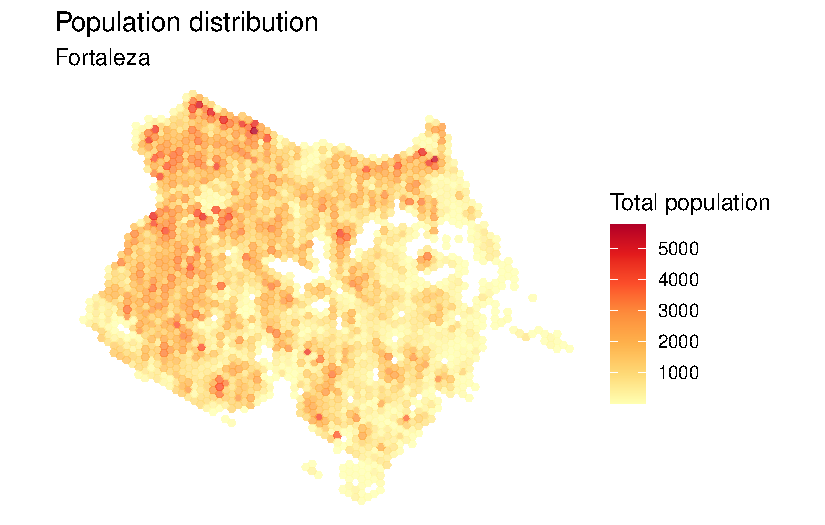
\includegraphics{./3_populacao_files/figure-pdf/plot population-1.pdf}

}

\end{figure}

\hypertarget{mapa-de-populauxe7uxe3o-por-cor}{%
\section{Mapa de população por
cor}\label{mapa-de-populauxe7uxe3o-por-cor}}

Além da informação sobre a população total em cada célula, o dados do
\texttt{aopdata} também permitem saber a quantidade de pessoas de
diferentes cores (variáveis \texttt{P002} a \texttt{P005}), sexo
(variáveis \texttt{P006} e \texttt{P007}) e faixas etárias (variáveis
\texttt{P010} à \texttt{P016}). O código abaixo ilustra como é simples
calcular a proporção de pessoas negras e brancas em cada hexágono e
visualizar esses dados num mapa.

\begin{Shaded}
\begin{Highlighting}[]
\NormalTok{pop\_b }\OtherTok{\textless{}{-}} \FunctionTok{ggplot}\NormalTok{() }\SpecialCharTok{+}
  \FunctionTok{geom\_sf}\NormalTok{(}\AttributeTok{data=}\FunctionTok{subset}\NormalTok{(df, P001 }\SpecialCharTok{\textgreater{}}\DecValTok{0}\NormalTok{), }\FunctionTok{aes}\NormalTok{(}\AttributeTok{fill=}\NormalTok{P003 }\SpecialCharTok{/}\NormalTok{ P001), }\AttributeTok{color=}\ConstantTok{NA}\NormalTok{, }\AttributeTok{alpha=}\NormalTok{.}\DecValTok{8}\NormalTok{) }\SpecialCharTok{+}
  \FunctionTok{scale\_fill\_distiller}\NormalTok{(}\AttributeTok{palette =} \StringTok{"RdPu"}\NormalTok{, }\AttributeTok{direction =} \DecValTok{1}\NormalTok{, }\AttributeTok{labels =}\NormalTok{ percent, }\AttributeTok{limits=}\FunctionTok{c}\NormalTok{(}\DecValTok{0}\NormalTok{, }\DecValTok{1}\NormalTok{))}\SpecialCharTok{+}
  \FunctionTok{labs}\NormalTok{(}\AttributeTok{title=}\StringTok{\textquotesingle{}Proportion of black population\textquotesingle{}}\NormalTok{, }\AttributeTok{fill=}\StringTok{"Black pop."}\NormalTok{) }\SpecialCharTok{+}
  \FunctionTok{theme\_void}\NormalTok{()}

\NormalTok{pop\_w }\OtherTok{\textless{}{-}} \FunctionTok{ggplot}\NormalTok{() }\SpecialCharTok{+}
  \FunctionTok{geom\_sf}\NormalTok{(}\AttributeTok{data=}\FunctionTok{subset}\NormalTok{(df, P001 }\SpecialCharTok{\textgreater{}}\DecValTok{0}\NormalTok{), }\FunctionTok{aes}\NormalTok{(}\AttributeTok{fill=}\NormalTok{P002 }\SpecialCharTok{/}\NormalTok{ P001), }\AttributeTok{color=}\ConstantTok{NA}\NormalTok{, }\AttributeTok{alpha=}\NormalTok{.}\DecValTok{8}\NormalTok{) }\SpecialCharTok{+}
  \FunctionTok{scale\_fill\_distiller}\NormalTok{(}\AttributeTok{palette =} \StringTok{"YlGnBu"}\NormalTok{, }\AttributeTok{direction =} \DecValTok{1}\NormalTok{, }\AttributeTok{labels =}\NormalTok{ percent, }\AttributeTok{limits=}\FunctionTok{c}\NormalTok{(}\DecValTok{0}\NormalTok{, }\DecValTok{1}\NormalTok{))}\SpecialCharTok{+}
  \FunctionTok{labs}\NormalTok{(}\AttributeTok{title=}\StringTok{\textquotesingle{}Proportion of white population\textquotesingle{}}\NormalTok{, }\AttributeTok{fill=}\StringTok{"White pop."}\NormalTok{) }\SpecialCharTok{+}
  \FunctionTok{theme\_void}\NormalTok{()}

\CommentTok{\# plot figure}
\NormalTok{pop\_b }\SpecialCharTok{+}\NormalTok{ pop\_w}
\end{Highlighting}
\end{Shaded}

\begin{figure}[H]

{\centering 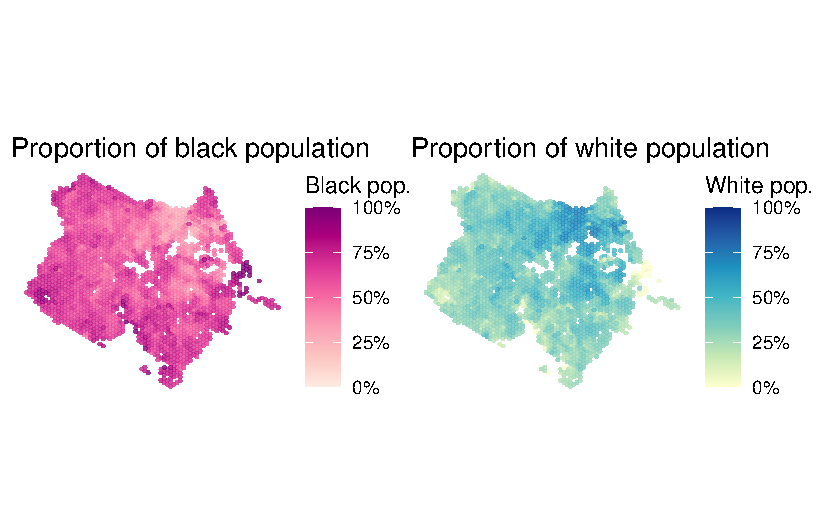
\includegraphics{./3_populacao_files/figure-pdf/plot race-1.pdf}

}

\end{figure}

\hypertarget{mapa-de-populauxe7uxe3o-por-renda}{%
\section{Mapa de população por
renda}\label{mapa-de-populauxe7uxe3o-por-renda}}

Os dados trazem também informação sobre a renda domiciliar per capita
média de cada hexágono (\texttt{R001}), e sua classificação em termos de
quintil (\texttt{R002}) e decil de renda (\texttt{R003}). Com esses
dados, é possível visualizar com o comando abaixo a distribuição
espacial dos diferentes níveis de renda da cidade.R

\begin{Shaded}
\begin{Highlighting}[]
\NormalTok{renda\_c }\OtherTok{\textless{}{-}} \FunctionTok{ggplot}\NormalTok{() }\SpecialCharTok{+}
  \FunctionTok{geom\_sf}\NormalTok{(}\AttributeTok{data=}\FunctionTok{subset}\NormalTok{(df, P001 }\SpecialCharTok{\textgreater{}}\DecValTok{0}\NormalTok{), }\FunctionTok{aes}\NormalTok{(}\AttributeTok{fill=}\NormalTok{R001), }\AttributeTok{color=}\ConstantTok{NA}\NormalTok{, }\AttributeTok{alpha=}\NormalTok{.}\DecValTok{8}\NormalTok{) }\SpecialCharTok{+}
  \FunctionTok{scale\_fill\_distiller}\NormalTok{(}\AttributeTok{palette =} \StringTok{"YlOrRd"}\NormalTok{, }\AttributeTok{direction =} \DecValTok{1}\NormalTok{)}\SpecialCharTok{+}
  \FunctionTok{labs}\NormalTok{(}\AttributeTok{title=}\StringTok{\textquotesingle{}Renda domiciliar per capita média\textquotesingle{}}\NormalTok{, }\AttributeTok{fill=}\StringTok{"Renda em R$"}\NormalTok{) }\SpecialCharTok{+}
  \FunctionTok{theme\_void}\NormalTok{()}

\NormalTok{renda\_d }\OtherTok{\textless{}{-}} \FunctionTok{ggplot}\NormalTok{() }\SpecialCharTok{+}
  \FunctionTok{geom\_sf}\NormalTok{(}\AttributeTok{data=}\FunctionTok{subset}\NormalTok{(df, }\SpecialCharTok{!}\FunctionTok{is.na}\NormalTok{(R002)), }\FunctionTok{aes}\NormalTok{(}\AttributeTok{fill=}\FunctionTok{factor}\NormalTok{(R003)), }\AttributeTok{color=}\ConstantTok{NA}\NormalTok{, }\AttributeTok{alpha=}\NormalTok{.}\DecValTok{8}\NormalTok{) }\SpecialCharTok{+}
  \FunctionTok{scale\_fill\_brewer}\NormalTok{(}\AttributeTok{palette =} \StringTok{"RdBu"}\NormalTok{) }\SpecialCharTok{+}
  \FunctionTok{labs}\NormalTok{(}\AttributeTok{title=}\StringTok{\textquotesingle{}Decils de renda domiciliar per capita\textquotesingle{}}\NormalTok{, }\AttributeTok{fill=}\StringTok{"Decil de renda"}\NormalTok{) }\SpecialCharTok{+}
  \FunctionTok{theme\_void}\NormalTok{() }\SpecialCharTok{+}
  \FunctionTok{theme}\NormalTok{(}\AttributeTok{legend.key.size =} \FunctionTok{unit}\NormalTok{(.}\DecValTok{3}\NormalTok{, }\StringTok{\textquotesingle{}cm\textquotesingle{}}\NormalTok{))}

\CommentTok{\# plot figure}
\NormalTok{renda\_c }\SpecialCharTok{+}\NormalTok{ renda\_d}
\end{Highlighting}
\end{Shaded}

\begin{figure}[H]

{\centering 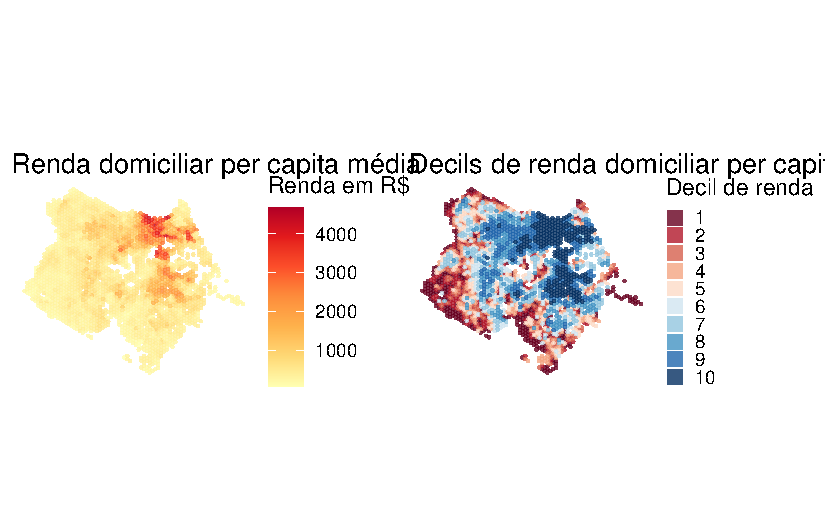
\includegraphics{./3_populacao_files/figure-pdf/plot income-1.pdf}

}

\end{figure}

\hypertarget{dados-de-distribuiuxe7uxe3o-espacial-de-oportunidades}{%
\chapter{Dados de distribuição espacial de
oportunidades}\label{dados-de-distribuiuxe7uxe3o-espacial-de-oportunidades}}

\hypertarget{download-dos-dados-1}{%
\section{Download dos dados}\label{download-dos-dados-1}}

O pacote \texttt{aopdata} também permite baixar, para todas cidades
incluídas no projeto, dados anuais da distribuição espacial de empregos
(de baixa, média e alta escolaridade), estabelecimentos de saúde (de
baixa, média e alta complexidade), escolas pública (ensino infantil,
fundamental e médio), e de centros de referência de assistência social
(Cras).

Todos esses dados podem ser baixados com a função
\texttt{read\_landuse()}, que funciona da mesma maneira que a função
\texttt{read\_population()}. Você só precisa indicar nos parâmetros da
função qual cidade (\texttt{city}) e ano (\texttt{year}) devem ser
baixados, além de apontar se deseja que os dados contenham as
informações espaciais dos hexágonos (\texttt{geometry\ =\ TRUE}).

Neste exemplo, abaixo, nós mostramos como baixar os dados de uso do solo
no ano de 2019 para Belo Horizonte. Note que essa função automaticamente
já baixa também os dados de população, automaticamente.

\begin{Shaded}
\begin{Highlighting}[]
\FunctionTok{library}\NormalTok{(aopdata)}
\end{Highlighting}
\end{Shaded}

\begin{verbatim}
Warning: package 'aopdata' was built under R version 4.1.3
\end{verbatim}

\begin{Shaded}
\begin{Highlighting}[]
\CommentTok{\# download aop land use data}
\NormalTok{df }\OtherTok{\textless{}{-}} \FunctionTok{read\_landuse}\NormalTok{(}\AttributeTok{city=}\StringTok{\textquotesingle{}Belo Horizonte\textquotesingle{}}\NormalTok{,}
                      \AttributeTok{year=}\DecValTok{2019}\NormalTok{,}
                      \AttributeTok{geometry =} \ConstantTok{TRUE}\NormalTok{,}
                      \AttributeTok{showProgress =} \ConstantTok{FALSE}\NormalTok{)}
\end{Highlighting}
\end{Shaded}

\begin{verbatim}
Downloading land use data for the year 2019
\end{verbatim}

\begin{verbatim}
Downloading population data for the year 2010
\end{verbatim}

\begin{Shaded}
\begin{Highlighting}[]
\FunctionTok{head}\NormalTok{(df)}
\end{Highlighting}
\end{Shaded}

\begin{verbatim}
Simple feature collection with 6 features and 39 fields
Geometry type: POLYGON
Dimension:     XY
Bounding box:  xmin: -43.87914 ymin: -19.86084 xmax: -43.85906 ymax: -19.82421
Geodetic CRS:  WGS 84
           id_hex abbrev_muni      name_muni code_muni P001 P002 P003 P004 P005
1 89a881345a3ffff         bho Belo Horizonte   3106200    0    0    0    0    0
2 89a881345a7ffff         bho Belo Horizonte   3106200    0    0    0    0    0
3 89a881345b7ffff         bho Belo Horizonte   3106200    0    0    0    0    0
4 89a88136103ffff         bho Belo Horizonte   3106200  508  141  353    4   10
5 89a88136107ffff         bho Belo Horizonte   3106200  428  114  304    3    7
6 89a8813610bffff         bho Belo Horizonte   3106200  399  111  277    3    8
  P006 P007 P010 P011 P012 P013 P014 P015 P016  R001 R002 R003 year T001 T002
1    0    0    0    0    0    0    0    0    0    NA   NA   NA 2019    0    0
2    0    0    0    0    0    0    0    0    0    NA   NA   NA 2019    0    0
3    0    0    0    0    0    0    0    0    0    NA   NA   NA 2019    0    0
4  253  255   53   86   30   43  176  110   10 502.9    2    3 2019  100   17
5  210  218   42   72   27   38  142   98    9 491.8    2    3 2019   44   19
6  203  196   42   68   24   34  138   86    7 502.8    2    3 2019  104   31
  T003 T004 E001 E002 E003 E004 M001 M002 M003 M004 S001 S002 S003 S004 C001
1    0    0    0    0    0    0    0    0    0    0    0    0    0    0    0
2    0    0    0    0    0    0    0    0    0    0    0    0    0    0    0
3    0    0    0    0    0    0    0    0    0    0    0    0    0    0    0
4   72   11    1    1    0    0  321  321    0    0    0    0    0    0    0
5   23    2    0    0    0    0    0    0    0    0    0    0    0    0    0
6   58   15    1    0    1    0  817    0  817    0    0    0    0    0    0
                        geometry
1 POLYGON ((-43.86011 -19.829...
2 POLYGON ((-43.86313 -19.827...
3 POLYGON ((-43.86321 -19.830...
4 POLYGON ((-43.8731 -19.8608...
5 POLYGON ((-43.87612 -19.859...
6 POLYGON ((-43.87001 -19.859...
\end{verbatim}

Antes de visualizar os dados de uso do solo nas próxima seções, vamos
carregar algumas bibliotecas de visualização e manipulação de dados.

\begin{Shaded}
\begin{Highlighting}[]
\CommentTok{\# load libraries}
\FunctionTok{library}\NormalTok{(patchwork)}
\FunctionTok{library}\NormalTok{(ggplot2)}
\FunctionTok{library}\NormalTok{(scales)}
\FunctionTok{library}\NormalTok{(sf)}
\end{Highlighting}
\end{Shaded}

\hypertarget{mapa-de-empregos}{%
\section{Mapa de empregos}\label{mapa-de-empregos}}

Como nos exemplos anteriores, é possível visualizar o mapa de
distribuição espacial de empregos usando o pacote \texttt{ggplot2} com o
código abaixo:

\begin{Shaded}
\begin{Highlighting}[]
\FunctionTok{ggplot}\NormalTok{() }\SpecialCharTok{+}
  \FunctionTok{geom\_sf}\NormalTok{(}\AttributeTok{data=}\NormalTok{df, }\FunctionTok{aes}\NormalTok{(}\AttributeTok{fill=}\NormalTok{T001), }\AttributeTok{color=}\ConstantTok{NA}\NormalTok{, }\AttributeTok{alpha=}\NormalTok{.}\DecValTok{9}\NormalTok{) }\SpecialCharTok{+}
  \FunctionTok{scale\_fill\_distiller}\NormalTok{(}\AttributeTok{palette =} \StringTok{"YlGnBu"}\NormalTok{, }\AttributeTok{direction =} \DecValTok{1}\NormalTok{) }\SpecialCharTok{+}
  \FunctionTok{labs}\NormalTok{(}\AttributeTok{title=}\StringTok{\textquotesingle{}Distribuição espacial de empregos\textquotesingle{}}\NormalTok{, }
       \AttributeTok{subtitle =} \StringTok{\textquotesingle{}Belo Horizonte\textquotesingle{}}\NormalTok{, }\AttributeTok{fill=}\StringTok{"N. de empregos"}\NormalTok{) }\SpecialCharTok{+}
  \FunctionTok{theme\_void}\NormalTok{()}
\end{Highlighting}
\end{Shaded}

\begin{figure}[H]

{\centering 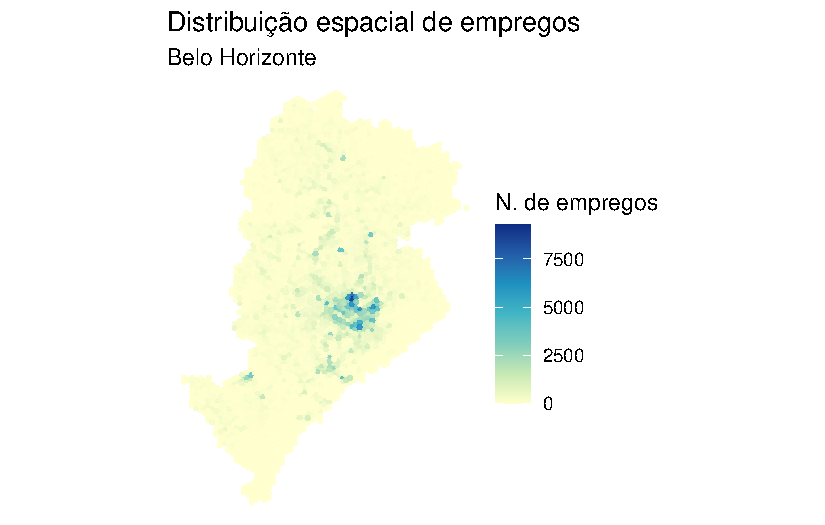
\includegraphics{./4_uso_solo_files/figure-pdf/plot jobs-1.pdf}

}

\end{figure}

\hypertarget{mapa-de-escolas}{%
\section{Mapa de escolas}\label{mapa-de-escolas}}

As variáveis que indicam o número de escolas em cada célula são aquelas
que começam com a letra \texttt{E\_\_}. Neste exemplo abaixo, nós
mapeamos a distribuição espacial de todas escolas de Belo Horizonte a
partir da variável \texttt{E001}.

\begin{Shaded}
\begin{Highlighting}[]
\FunctionTok{ggplot}\NormalTok{() }\SpecialCharTok{+}
  \FunctionTok{geom\_sf}\NormalTok{(}\AttributeTok{data=}\NormalTok{df, }\FunctionTok{aes}\NormalTok{(}\AttributeTok{fill=}\FunctionTok{as.factor}\NormalTok{(E001)), }\AttributeTok{color=}\ConstantTok{NA}\NormalTok{, }\AttributeTok{alpha=}\NormalTok{.}\DecValTok{9}\NormalTok{) }\SpecialCharTok{+}
   \FunctionTok{scale\_fill\_brewer}\NormalTok{(}\AttributeTok{palette =} \StringTok{"YlGnBu"}\NormalTok{, }\AttributeTok{direction =} \DecValTok{1}\NormalTok{) }\SpecialCharTok{+}
  \FunctionTok{labs}\NormalTok{(}\AttributeTok{title=}\StringTok{\textquotesingle{}Distribuição espacial de escolas\textquotesingle{}}\NormalTok{, }
       \AttributeTok{subtitle =} \StringTok{\textquotesingle{}Belo Horizonte\textquotesingle{}}\NormalTok{, }\AttributeTok{fill=}\StringTok{"N. de escolas"}\NormalTok{) }\SpecialCharTok{+}
  \FunctionTok{theme\_void}\NormalTok{()}
\end{Highlighting}
\end{Shaded}

\begin{figure}[H]

{\centering 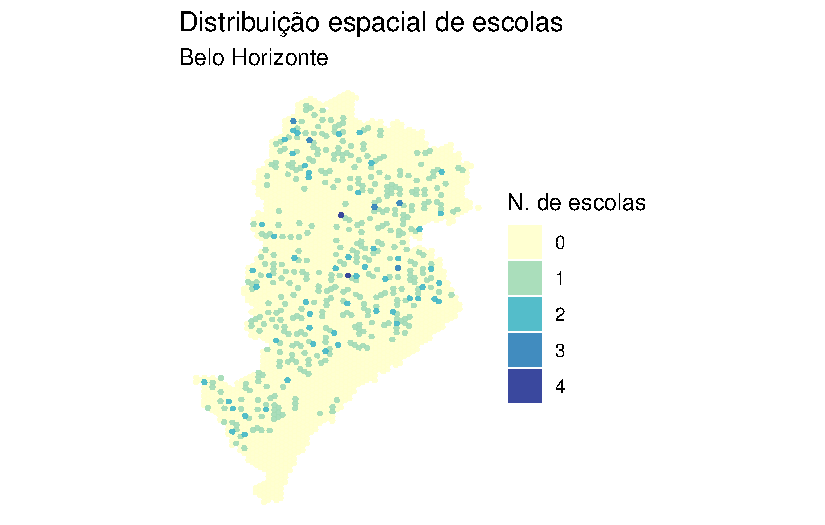
\includegraphics{./4_uso_solo_files/figure-pdf/plot schools-1.pdf}

}

\end{figure}

\hypertarget{mapa-de-estabelecimentos-de-sauxfade}{%
\section{Mapa de estabelecimentos de
saúde}\label{mapa-de-estabelecimentos-de-sauxfade}}

Para analisar a distribuição espacial de estabelecimentos de saúde, você
deve analisar as variáveis que começam com a letra \texttt{S\_\_\_}. O
código abaixo nos permite comparar a distribuição espacial de
estabelecimentos de saúde de baixa complexidade (\texttt{S002}) e alta
complexidade (\texttt{S004}).

\begin{Shaded}
\begin{Highlighting}[]
\NormalTok{sau\_b }\OtherTok{\textless{}{-}} \FunctionTok{ggplot}\NormalTok{() }\SpecialCharTok{+}
          \FunctionTok{geom\_sf}\NormalTok{(}\AttributeTok{data=}\NormalTok{df, }\FunctionTok{aes}\NormalTok{(}\AttributeTok{fill=}\FunctionTok{as.factor}\NormalTok{(S002)), }\AttributeTok{color=}\ConstantTok{NA}\NormalTok{, }\AttributeTok{alpha=}\NormalTok{.}\DecValTok{9}\NormalTok{) }\SpecialCharTok{+}
          \FunctionTok{scale\_fill\_brewer}\NormalTok{(}\AttributeTok{palette =} \StringTok{"YlGnBu"}\NormalTok{, }\AttributeTok{direction =} \DecValTok{1}\NormalTok{, }\AttributeTok{limits=}\FunctionTok{factor}\NormalTok{(}\DecValTok{0}\SpecialCharTok{:}\DecValTok{4}\NormalTok{)) }\SpecialCharTok{+}
          \FunctionTok{labs}\NormalTok{(}\AttributeTok{title=}\StringTok{\textquotesingle{}Estabelecimentos de saúde\textquotesingle{}}\NormalTok{, }\AttributeTok{subtitle =} \StringTok{\textquotesingle{}Baixa complexidade\textquotesingle{}}\NormalTok{,}
               \AttributeTok{fill=}\StringTok{"N. de estabelecimentos"}\NormalTok{) }\SpecialCharTok{+}
          \FunctionTok{theme\_void}\NormalTok{()}

\NormalTok{sau\_a }\OtherTok{\textless{}{-}} \FunctionTok{ggplot}\NormalTok{() }\SpecialCharTok{+}
          \FunctionTok{geom\_sf}\NormalTok{(}\AttributeTok{data=}\NormalTok{df, }\FunctionTok{aes}\NormalTok{(}\AttributeTok{fill=}\FunctionTok{as.factor}\NormalTok{(S004)), }\AttributeTok{color=}\ConstantTok{NA}\NormalTok{, }\AttributeTok{alpha=}\NormalTok{.}\DecValTok{9}\NormalTok{) }\SpecialCharTok{+}
          \FunctionTok{scale\_fill\_brewer}\NormalTok{(}\AttributeTok{palette =} \StringTok{"YlGnBu"}\NormalTok{, }\AttributeTok{direction =} \DecValTok{1}\NormalTok{, }\AttributeTok{limits=}\FunctionTok{factor}\NormalTok{(}\DecValTok{0}\SpecialCharTok{:}\DecValTok{4}\NormalTok{)) }\SpecialCharTok{+}
          \FunctionTok{labs}\NormalTok{(}\AttributeTok{title=}\StringTok{\textquotesingle{}Estabelecimentos de saúde\textquotesingle{}}\NormalTok{, }\AttributeTok{subtitle =} \StringTok{\textquotesingle{}Alta complexidade\textquotesingle{}}\NormalTok{,}
               \AttributeTok{fill=}\StringTok{"N. de estabelecimentos"}\NormalTok{) }\SpecialCharTok{+}
          \FunctionTok{theme\_void}\NormalTok{()}

\CommentTok{\# plot maps}
\NormalTok{sau\_b  }\SpecialCharTok{+}\NormalTok{ sau\_a  }\SpecialCharTok{+} \FunctionTok{plot\_layout}\NormalTok{(}\AttributeTok{guides =} \StringTok{\textquotesingle{}collect\textquotesingle{}}\NormalTok{)}
\end{Highlighting}
\end{Shaded}

\begin{figure}[H]

{\centering 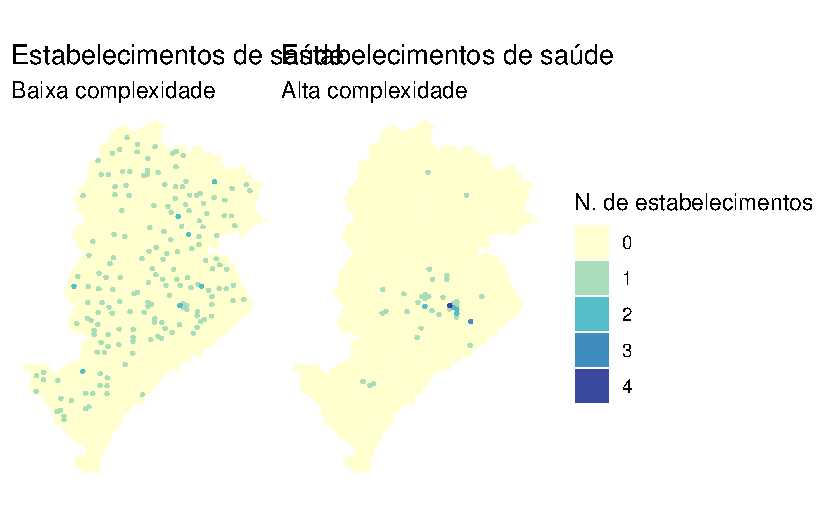
\includegraphics{./4_uso_solo_files/figure-pdf/plot health facilities-1.pdf}

}

\end{figure}

\hypertarget{mapa-de-cras}{%
\section{Mapa de CRAS}\label{mapa-de-cras}}

Por fim, a distribuição espacial dos Centros de Referência de
Assistência Social (Cras) pode ser analisada com a variável
\texttt{C001}.

\begin{Shaded}
\begin{Highlighting}[]
\FunctionTok{ggplot}\NormalTok{() }\SpecialCharTok{+}
  \FunctionTok{geom\_sf}\NormalTok{(}\AttributeTok{data=}\NormalTok{df, }\FunctionTok{aes}\NormalTok{(}\AttributeTok{fill=}\FunctionTok{as.factor}\NormalTok{(C001)), }\AttributeTok{color=}\ConstantTok{NA}\NormalTok{, }\AttributeTok{alpha=}\NormalTok{.}\DecValTok{9}\NormalTok{) }\SpecialCharTok{+}
   \FunctionTok{scale\_fill\_brewer}\NormalTok{(}\AttributeTok{palette =} \StringTok{"YlGnBu"}\NormalTok{, }\AttributeTok{direction =} \DecValTok{1}\NormalTok{) }\SpecialCharTok{+}
  \FunctionTok{labs}\NormalTok{(}\AttributeTok{title=}\StringTok{\textquotesingle{}Centros de Referência de Assistência Social (Cras)\textquotesingle{}}\NormalTok{, }
       \AttributeTok{subtitle =} \StringTok{\textquotesingle{}Belo Horizonte\textquotesingle{}}\NormalTok{, }\AttributeTok{fill=}\StringTok{"N. de Cras"}\NormalTok{) }\SpecialCharTok{+}
  \FunctionTok{theme\_void}\NormalTok{()}
\end{Highlighting}
\end{Shaded}

\begin{figure}[H]

{\centering 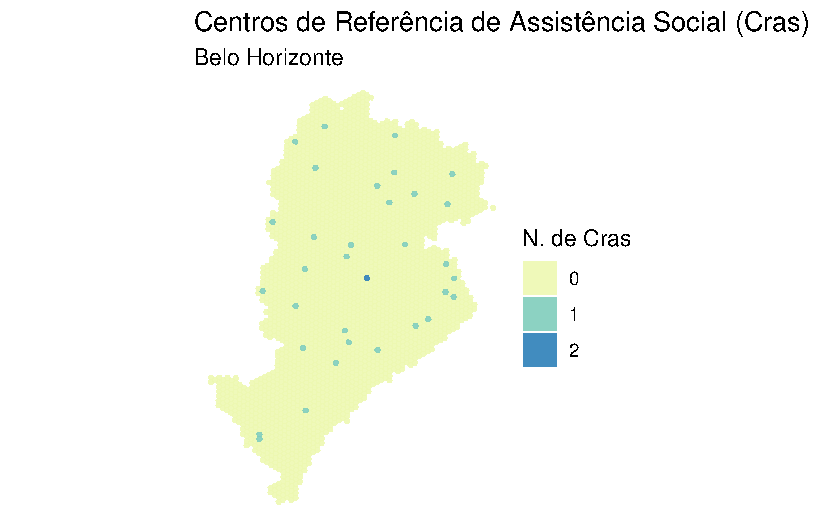
\includegraphics{./4_uso_solo_files/figure-pdf/plot cras-1.pdf}

}

\end{figure}

\hypertarget{estimativas-e-mapas-de-acessibilidade}{%
\chapter{Estimativas e mapas de
acessibilidade}\label{estimativas-e-mapas-de-acessibilidade}}

\hypertarget{download-dos-dados-2}{%
\section{Download dos dados}\label{download-dos-dados-2}}

Finalmente, o pacote \texttt{aopdata} também permite baixar, para todas
cidades incluídas no projeto, estimativas anuais de acesso a empregos,
serviços saúde, educação e assistência social por modo de transporte

Todos esses dados podem ser baixados com a função
\texttt{read\_access()}, que funciona da mesma maneira que as funções
\texttt{read\_population()} e \texttt{read\_landuse()} apresentadas nos
capítulos anteriores. Aqui, no entanto, além de indicar a cidade
(\texttt{city}) e o ano (\texttt{year}) de referência para baixar os
dados, você também precisa informar qual o modo de transporte
(\texttt{mode}) será baixado e se você quer estimativas de
acessibilidade no horário de pico (\texttt{peak\ =\ TRUE}) ou fora-pico
(\texttt{peak\ =\ TRUE}). Esses dados representam a acessibilidade
mediana do período de pico (entre 6h e 8h) e fora-pico (entre 14h e
16h).

Neste exemplo, abaixo, nós mostramos como baixar os dados de uso de
acessibilidade urbana no ano de 2019 para São Paulo no período de pico.
Nesse exemplo, nós baixamos tanto as estimativas de acessibilidade por
automóvel quanto por transporte público, e empilhamos os dados num único
\texttt{data.frame}. Note que essa função automaticamente já baixa
também os dados de população e de uso do solo, automaticamente.

\begin{Shaded}
\begin{Highlighting}[]
\FunctionTok{library}\NormalTok{(aopdata)}

\CommentTok{\# download aop accessibility data}
\NormalTok{df\_pt }\OtherTok{\textless{}{-}} \FunctionTok{read\_access}\NormalTok{(}
  \AttributeTok{city=}\StringTok{\textquotesingle{}São Paulo\textquotesingle{}}\NormalTok{,}
  \AttributeTok{mode=}\StringTok{\textquotesingle{}public\_transport\textquotesingle{}}\NormalTok{,}
  \AttributeTok{year=}\DecValTok{2019}\NormalTok{,}
  \AttributeTok{peak =} \ConstantTok{TRUE}\NormalTok{,}
  \AttributeTok{geometry =} \ConstantTok{TRUE}\NormalTok{,}
  \AttributeTok{showProgress =} \ConstantTok{FALSE}
\NormalTok{)}

\NormalTok{df\_car }\OtherTok{\textless{}{-}} \FunctionTok{read\_access}\NormalTok{(}
  \AttributeTok{city=}\StringTok{\textquotesingle{}São Paulo\textquotesingle{}}\NormalTok{,}
  \AttributeTok{mode=}\StringTok{\textquotesingle{}car\textquotesingle{}}\NormalTok{,}
  \AttributeTok{year=}\DecValTok{2019}\NormalTok{,}
  \AttributeTok{peak =} \ConstantTok{TRUE}\NormalTok{,}
  \AttributeTok{geometry =} \ConstantTok{TRUE}\NormalTok{,}
  \AttributeTok{showProgress =} \ConstantTok{FALSE}
\NormalTok{)}

\CommentTok{\# row bind into a single data.frame}
\NormalTok{df }\OtherTok{\textless{}{-}} \FunctionTok{rbind}\NormalTok{(df\_pt, df\_car)}
\FunctionTok{head}\NormalTok{(df)}
\end{Highlighting}
\end{Shaded}

\begin{verbatim}
Simple feature collection with 6 features and 205 fields
Geometry type: POLYGON
Dimension:     XY
Bounding box:  xmin: -46.63863 ymin: -23.71413 xmax: -46.62834 ymax: -23.70485
Geodetic CRS:  WGS 84
           id_hex abbrev_muni name_muni code_muni year P001 P002 P003 P004 P005
1 89a81000003ffff         spo Sao Paulo   3550308 2019  322  127  190    0    5
2 89a81000007ffff         spo Sao Paulo   3550308 2019   16    3   13    0    0
3 89a8100000bffff         spo Sao Paulo   3550308 2019 2386 1142 1232    2   10
4 89a8100000fffff         spo Sao Paulo   3550308 2019  885  260  622    0    3
5 89a81000013ffff         spo Sao Paulo   3550308 2019  725  340  380    0    5
6 89a81000017ffff         spo Sao Paulo   3550308 2019  211  110   98    0    3
  P006 P007 P010 P011 P012 P013 P014 P015 P016  R001 R002 R003 T001 T002 T003
1  158  164   33   63   28   35   85   75    3 477.6    2    3   72   19   50
2    9    7    2    2    2    3    2    5    0  65.7    1    1    0    0    0
3 1216 1170  247  410  174  269  682  572   32 377.2    1    1   52    6   24
4  460  425   96  124   88  127  175  266    9 363.9    1    1    0    0    0
5  371  354   85  129   51   78  196  173   13 503.5    2    3    0    0    0
6  104  107   20   33   16   25   52   59    6 687.9    3    6  113   18   65
  T004 E001 E002 E003 E004 M001 M002 M003 M004 S001 S002 S003 S004 C001
1    3    0    0    0    0    0    0    0    0    0    0    0    0    0
2    0    0    0    0    0    0    0    0    0    0    0    0    0    0
3   22    0    0    0    0    0    0    0    0    0    0    0    0    0
4    0    0    0    0    0    0    0    0    0    0    0    0    0    0
5    0    0    0    0    0    0    0    0    0    0    0    0    0    0
6   30    2    0    2    1 1477    0 1168  309    0    0    0    0    0
              mode peak CMATT15 CMATB15 CMATM15 CMATA15 CMAST15 CMASB15 CMASM15
1 public_transport    1     315      71     175      69       0       0       0
2 public_transport    1     313      70     174      69       0       0       0
3 public_transport    1     229      43     161      25       2       2       2
4 public_transport    1     551     123     343      85       3       3       3
5 public_transport    1     421      90     262      69       2       2       2
6 public_transport    1     312      76     187      49       0       0       0
  CMASA15 CMAET15 CMAEI15 CMAEF15 CMAEM15 CMAMT15 CMAMI15 CMAMF15 CMAMM15
1       0       2       0       2       1    1477       0    1168     309
2       0       2       0       2       1    1477       0    1168     309
3       0       0       0       0       0       0       0       0       0
4       0       4       1       3       2    3132     460    1965     707
5       0       2       0       2       1    1477       0    1168     309
6       0       2       0       2       1    1477       0    1168     309
  CMACT15 CMPPT15 CMPPH15 CMPPM15 CMPPB15 CMPPA15 CMPPI15 CMPPN15 CMPP0005I15
1       0    4895    2428    2467    2238      27       2    2628         505
2       0    4895    2428    2467    2238      27       2    2628         505
3       0    9537    4645    4892    4685      64       3    4785         872
4       0   13109    6331    6778    6453      61       8    6587        1088
5       0    4934    2452    2482    2368      48       0    2518         461
6       0    3199    1608    1591    1567      20       0    1612         317
  CMPP0614I15 CMPP1518I15 CMPP1924I15 CMPP2539I15 CMPP4069I15 CMPP70I15 CMATT30
1         809         371         566        1313        1247        84    4797
2         809         371         566        1313        1247        84    4228
3        1538         726        1138        2550        2539       174    2648
4        2012         967        1575        3383        3783       301    6200
5         749         373         587        1271        1372       121    5773
6         487         239         374         807         891        84    6608
  CMATB30 CMATM30 CMATA30 CMAST30 CMASB30 CMASM30 CMASA30 CMAET30 CMAEI30
1    1293    2789     715       5       5       5       0      18       5
2    1170    2452     606       4       4       4       0      13       4
3     714    1526     408       4       4       4       0       9       2
4    1598    3641     961       5       5       5       0      19       6
5    1589    3271     913       5       5       5       0      18       5
6    1821    3659    1128       6       6       6       0      22       5
  CMAEF30 CMAEM30 CMAMT30 CMAMI30 CMAMF30 CMAMM30 CMACT30 CMPPT30 CMPPH30
1      13       4   15148    2409   10765    1974       1   59041   28457
2       9       3   10497    1949    6931    1617       1   40049   19392
3       7       3    7222    1069    5137    1016       1   59792   28974
4      13       5   15710    2527   10551    2632       2  101380   48709
5      13       4   15148    2409   10765    1974       1   81985   39473
6      17       5   19547    2409   14343    2795       1   83186   40111
  CMPPM30 CMPPB30 CMPPA30 CMPPI30 CMPPN30 CMPP0005I30 CMPP0614I30 CMPP1518I30
1   30584   28535     446      29   30031        5263        8809        4111
2   20657   19159     273      14   20603        3610        6061        2866
3   30818   28424     365      25   30978        5376        9204        4241
4   52671   47601     955      66   52758        9076       15239        6971
5   42512   39784     695      49   41457        7189       12278        5675
6   43075   40359     728      51   42048        7302       12371        5749
  CMPP1924I30 CMPP2539I30 CMPP4069I30 CMPP70I30 CMATT60 CMATB60 CMATM60 CMATA60
1        6817       15664       16733      1644   96195   18711   54773   22711
2        4673       10486       11274      1079   72810   14161   40949   17700
3        6927       15859       16646      1539  147237   26399   82208   38630
4       11658       27259       28303      2874  107938   21292   61768   24878
5        9311       21712       23351      2469  161353   28971   91687   40695
6        9459       22070       23710      2525  158016   28997   91280   37739
  CMAST60 CMASB60 CMASM60 CMASA60 CMAET60 CMAEI60 CMAEF60 CMAEM60 CMAMT60
1      50      38      48       6     120      40      76      29   87761
2      40      34      39       2     108      36      68      28   79902
3      57      45      56       5     135      45      88      30   93958
4      56      43      54       6     128      42      82      31   92799
5      59      44      57       7     141      47      90      32   97925
6      56      43      54       6     139      47      87      32   96281
  CMAMI60 CMAMF60 CMAMM60 CMACT60 CMPPT60 CMPPH60 CMPPM60 CMPPB60 CMPPA60
1   15059   56558   16144       5  547471  259971  287500  277734   11134
2   14014   50455   15433       5  501558  238550  263008  247962    8781
3   16318   61918   15722       6  633994  299454  334540  339064   19838
4   15615   60049   17135       5  689942  325560  364382  378571   21810
5   16744   63838   17343       6  666492  314759  351733  360532   20661
6   16812   62265   17204       6  632529  299225  333304  334655   17957
  CMPPI60 CMPPN60 CMPP0005I60 CMPP0614I60 CMPP1518I60 CMPP1924I60 CMPP2539I60
1     407  258196       44866       76195       34899       59393      146870
2     383  244432       41903       71199       32501       54873      134759
3     473  274619       49586       83666       38585       67298      169669
4     496  289065       53223       89680       41446       72354      184045
5     483  284816       51720       87430       40333       70418      178015
6     451  279466       49804       84545       38888       67458      168928
  CMPP4069I60 CMPP70I60 CMATT90 CMATB90 CMATM90 CMATA90 CMAST90 CMASB90 CMASM90
1      162048     23200 1168463  166686  577124  424653     169     111     160
2      146361     19962 1088120  153982  540566  393572     160     107     152
3      194234     30956 1428750  211239  719220  498291     190     119     179
4      214049     35145 1362473  191461  669950  501062     182     117     172
5      205504     33072 1443193  211449  723001  508743     203     131     191
6      192822     30084 1406215  203383  701014  501818     204     132     193
  CMASA90 CMAET90 CMAEI90 CMAEF90 CMAEM90 CMAMT90 CMAMI90 CMAMF90 CMAMM90
1      42     337     107     207      92  218542   30864  131526   56152
2      39     328     105     201      90  213963   30365  128917   54681
3      50     370     123     222     101  232126   34693  138061   59372
4      46     355     117     214      92  223492   32779  134438   56275
5      51     415     136     248     114  264729   38719  158252   67758
6      51     415     137     247     114  266946   39578  159137   68231
  CMACT90 CMPPT90 CMPPH90 CMPPM90 CMPPB90 CMPPA90 CMPPI90 CMPPN90 CMPP0005I90
1      10 1697502  790958  906544 1113577   80011    1336  502578      111963
2       9 1617428  753988  863440 1054271   74800    1240  487117      107419
3      10 1918445  894649 1023796 1274988   90290    1602  551565      125137
4      10 2096063  978494 1117569 1384576   94542    2065  614880      138110
5      12 2027043  946208 1080835 1333715   91633    1714  599981      133501
6      12 1950319  910888 1039431 1272271   88334    1558  588156      129637
  CMPP0614I90 CMPP1518I90 CMPP1924I90 CMPP2539I90 CMPP4069I90 CMPP70I90
1      183412       87698      165449      454122      573567    121291
2      176240       84154      157827      432825      545306    113657
3      204140       97829      187004      513061      650643    140631
4      225800      107835      205069      561408      707435    150406
5      218843      104726      198411      541774      684520    145268
6      212862      101535      191408      521731      655761    137385
  CMATT120 CMATB120 CMATM120 CMATA120 CMAST120 CMASB120 CMASM120 CMASA120
1  2136716   328724  1094450   713542      357      235      338       82
2  2095040   321900  1068319   704821      355      235      337       80
3  2203072   344047  1136019   723006      374      243      356       86
4  2494268   397258  1308021   788989      418      266      395       97
5  2275396   357833  1177979   739584      401      265      381       90
6  2195795   342423  1130056   723316      387      257      367       88
  CMAET120 CMAEI120 CMAEF120 CMAEM120 CMAMT120 CMAMI120 CMAMF120 CMAMM120
1      821      288      481      221   518042    83000   313683   121359
2      815      288      479      216   516846    83610   313657   119579
3      855      293      508      230   532772    82410   323147   127215
4      976      340      576      260   610890    97742   369803   143345
5      948      333      559      251   600516    97066   367244   136206
6      942      334      554      254   604830    98765   368433   137632
  CMACT120 CMPPT120 CMPPH120 CMPPM120 CMPPB120 CMPPA120 CMPPI120 CMPPN120
1       20  4018897  1890513  2128384  2540395   134426     4039  1340037
2       20  3860887  1814742  2046145  2445536   130803     3868  1280680
3       21  4320562  2032079  2288483  2745882   142238     4320  1428122
4       24  4752649  2234731  2517918  3037441   153875     5098  1556235
5       22  4351102  2049261  2301841  2735091   140022     4377  1471612
6       21  4191716  1974700  2217016  2627575   136196     4172  1423773
  CMPP0005I120 CMPP0614I120 CMPP1518I120 CMPP1924I120 CMPP2539I120 CMPP4069I120
1       281477       467671       217602       408477      1084792      1300130
2       269676       448086       208699       391944      1041317      1251187
3       301337       501274       233530       439651      1163931      1400822
4       330744       549438       256378       484187      1277780      1541189
5       307070       511736       237911       444278      1173140      1401287
6       297029       494835       229726       427661      1129908      1348228
  CMPP70I120 TMIST TMISB TMISM TMISA TMIET TMIEI TMIEF TMIEM TMICT
1     258748    17    17    17    53   8.0    26   8.0   8.0    21
2     249978    21    21    21    55   9.0    28   9.0   9.0    23
3     280017    13    13    13    50  17.0    26  17.0  17.0    30
4     312933    13    13    13    53   7.0    13   7.0   7.0    28
5     275680    12    12    12    51   8.0    24   8.0   8.0    19
6     264329    16    16    16    49   5.8    22   5.8   5.8    16
                        geometry
1 POLYGON ((-46.63251 -23.711...
2 POLYGON ((-46.63552 -23.709...
3 POLYGON ((-46.62941 -23.709...
4 POLYGON ((-46.63242 -23.708...
5 POLYGON ((-46.6326 -23.7141...
6 POLYGON ((-46.63561 -23.712...
\end{verbatim}

Os nomes das variáveis (colunas) com estimativas de acessibilidade
também estão organizadas com códigos, como \texttt{CMAEF30},
\texttt{TMISB} ou \texttt{CMPPM60}. O nome das colunas com estimativas
de acessibilidade são a junção de três componentes: 1) Tipo de indicador
de acessibilidade 2) Tipo de oportunidade / pessoas 3) Tempo limite

\begin{enumerate}
\def\labelenumi{\arabic{enumi})}
\tightlist
\item
  O \textbf{tipo de indicador} de acessibilidade é indicado pelas
  primeiras 3 letras. O projeto AOP atualmente inclui três tipos de
  indicadores:
\end{enumerate}

\begin{itemize}
\tightlist
\item
  \texttt{CMA} Indicador de acessibilidade cumulativo ativo
\item
  \texttt{CMP} Indicador de acessibilidade cumulativo passivo\\
\item
  \texttt{TMI} Indicador de tempo mínimo até oportunidade mais próxima
\end{itemize}

\begin{enumerate}
\def\labelenumi{\arabic{enumi})}
\setcounter{enumi}{1}
\tightlist
\item
  O \textbf{tipo de atividade} é indicado pelas letras seguintes, no
  meio do nome da variável. O projeto AOP atualmente inclui diversos
  tipos de atividades:
\end{enumerate}

\begin{itemize}
\tightlist
\item
  \texttt{TT} Todos empregos
\item
  \texttt{TB} Empregos de baixa escolaridade
\item
  \texttt{TM} Empregos de média escolaridade
\item
  \texttt{TA} Empregos de alta escolaridade
\item
  \texttt{ST} Todos estabelecimentos de saúde
\item
  \texttt{SB} Estabelecimentos de saúde de baixa complexidade
\item
  \texttt{SM} Estabelecimentos de saúde de média complexidade
\item
  \texttt{SA} Estabelecimentos de saúde de alta complexidade
\item
  \ldots{} e assim por diante.
\end{itemize}

No caso do indicador de acessibilidade passiva (\texttt{CMP}), as letras
do meio do nome da variável indicam qual o grupo populacional de
referência.

\begin{itemize}
\tightlist
\item
  \texttt{PT} População total
\item
  \texttt{PH} População de homens
\item
  \texttt{PM} População de mulheres
\item
  \texttt{PB} População branca
\item
  \texttt{PN} População negra
\item
  \texttt{P1924I} População de 19 a 24 anos de idade
\item
  \texttt{P2539I} População de 25 a 39 anos de idade
\end{itemize}

\begin{enumerate}
\def\labelenumi{\arabic{enumi})}
\setcounter{enumi}{2}
\tightlist
\item
  O \textbf{tempo limite de viagem} é indicado pelos números no final do
  nome da variável. Esses números somente se aplicam para os indicadores
  de acessibildade cumulativa ativa (\texttt{CMA}) e passiva
  (\texttt{CMP}).
\end{enumerate}

\textbf{Exemplos:}

{CMA}{EF}{30}: Número de escolas de ensino fundamental acessíveis em até
30 minutos

{TMI}{SB}: Tempo de viagem até o estabelecimento de saúde mais próximo
com serviços de baixa complexidade

{CMP}{PM}{60}: Quantidade de mulheres que conseguem acessar determinado
hexágono em até 60 minutos

Lembre-se, a
\href{https://ipeagit.github.io/aopdata/articles/data_dic_pt.html}{descrição
completa do dicionário de variáveis está disponível no site to pacote
aopdata}.

A seguir, nós mostramos alguns exemplos de como visualizar essas
estimativas de acessibilidade.

\hypertarget{mapa-do-tempo-para-acessar-o-hospital-mais-pruxf3ximo}{%
\section{Mapa do tempo para acessar o hospital mais
próximo}\label{mapa-do-tempo-para-acessar-o-hospital-mais-pruxf3ximo}}

Neste exemplo, nós vamos comparar o nível de acessibilidade até
hospitais entre modos automóvel \emph{vs} transporte público. Para
analisar qual o tempo mínimo de viagem (\texttt{TMI}) até um hospital de
alta complexidade (\texttt{SA}), nós precisamos analisar a variável
\texttt{TMISA}. Com o código abaixo, nós carregamos as bibliotecas para
manipulação e visualização de dados, e visualizamos a distribuição
espacial dos valores de \texttt{TMISA} para ambos modos de transporte.

Note, no entanto, que os tempos de viagem por transporte público
costumam ser muito mais longos do que por automóvel. Então para
facilitar a visualização dos resultados, nós truncamos a distribuição
dos valores de \texttt{TMISA} em 60 minutos ou mais.

\begin{Shaded}
\begin{Highlighting}[]
\CommentTok{\# load libraries}
\FunctionTok{library}\NormalTok{(ggplot2)}
\FunctionTok{library}\NormalTok{(data.table)}
\FunctionTok{library}\NormalTok{(patchwork)}
\FunctionTok{library}\NormalTok{(scales)}
\FunctionTok{library}\NormalTok{(sf)}

\CommentTok{\# truncate max values to 60 min.}
\NormalTok{df}\SpecialCharTok{$}\NormalTok{TMISA }\OtherTok{\textless{}{-}} \FunctionTok{ifelse}\NormalTok{(df}\SpecialCharTok{$}\NormalTok{TMISA }\SpecialCharTok{\textgreater{}} \DecValTok{60}\NormalTok{, }\DecValTok{60}\NormalTok{, df}\SpecialCharTok{$}\NormalTok{TMISA) }

\CommentTok{\# plot}
\FunctionTok{ggplot}\NormalTok{() }\SpecialCharTok{+}
  \FunctionTok{geom\_sf}\NormalTok{(}\AttributeTok{data=}\FunctionTok{subset}\NormalTok{(df, }\SpecialCharTok{!}\FunctionTok{is.na}\NormalTok{(mode)), }\FunctionTok{aes}\NormalTok{(}\AttributeTok{fill=}\NormalTok{TMISA), }\AttributeTok{color=}\ConstantTok{NA}\NormalTok{, }\AttributeTok{alpha=}\NormalTok{.}\DecValTok{9}\NormalTok{) }\SpecialCharTok{+}
  \FunctionTok{scale\_fill\_viridis\_c}\NormalTok{(}\AttributeTok{option =} \StringTok{\textquotesingle{}cividis\textquotesingle{}}\NormalTok{, }\AttributeTok{direction =} \SpecialCharTok{{-}}\DecValTok{1}\NormalTok{,}
                       \AttributeTok{breaks =} \FunctionTok{seq}\NormalTok{(}\DecValTok{0}\NormalTok{,}\DecValTok{60}\NormalTok{,}\DecValTok{10}\NormalTok{),}
                       \AttributeTok{labels =} \FunctionTok{c}\NormalTok{(}\FunctionTok{seq}\NormalTok{(}\DecValTok{0}\NormalTok{,}\DecValTok{50}\NormalTok{,}\DecValTok{10}\NormalTok{), }\StringTok{"60+"}\NormalTok{)) }\SpecialCharTok{+}
  \FunctionTok{labs}\NormalTok{(}\AttributeTok{title=}\StringTok{\textquotesingle{}Tempo de viagem até hospital de alta complex. mais próximo\textquotesingle{}}\NormalTok{, }
       \AttributeTok{subtitle =} \StringTok{\textquotesingle{}São Paulo\textquotesingle{}}\NormalTok{, }\AttributeTok{fill=}\StringTok{"Tempo em}\SpecialCharTok{\textbackslash{}n}\StringTok{minutos"}\NormalTok{) }\SpecialCharTok{+}
  \FunctionTok{facet\_grid}\NormalTok{(.}\SpecialCharTok{\textasciitilde{}}\NormalTok{mode) }\SpecialCharTok{+}
  \FunctionTok{theme\_void}\NormalTok{()}
\end{Highlighting}
\end{Shaded}

\begin{figure}[H]

{\centering 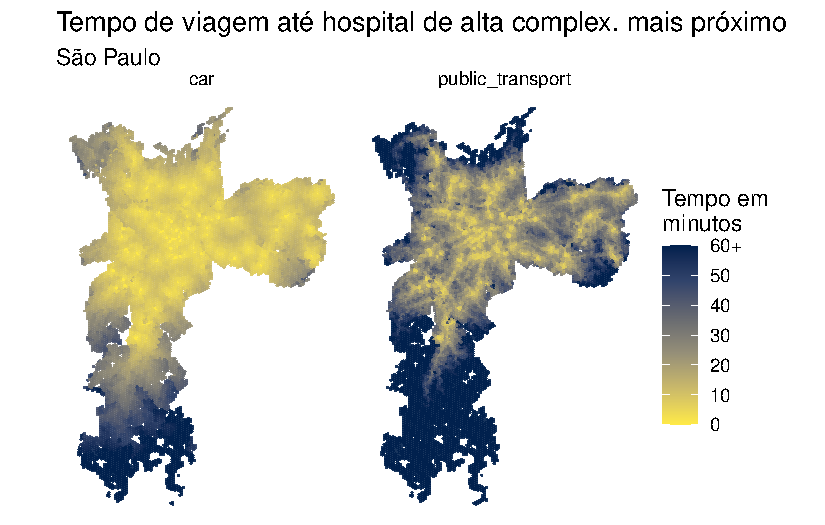
\includegraphics{./5_acessibilidade_files/figure-pdf/plot TMISA by car and pt-1.pdf}

}

\end{figure}

\hypertarget{mapa-da-quantidade-de-oportunidades-acessuxedveis}{%
\section{Mapa da quantidade de oportunidades
acessíveis}\label{mapa-da-quantidade-de-oportunidades-acessuxedveis}}

\begin{Shaded}
\begin{Highlighting}[]
\CommentTok{\# limits for legend scale}
\NormalTok{value\_limits }\OtherTok{\textless{}{-}} \FunctionTok{c}\NormalTok{(}\DecValTok{0}\NormalTok{, }\FunctionTok{max}\NormalTok{(df\_pt}\SpecialCharTok{$}\NormalTok{CMATT90, }\AttributeTok{na.rm=}\NormalTok{T)}\SpecialCharTok{/}\DecValTok{1000}\NormalTok{)}

\CommentTok{\# create maps}
\NormalTok{fig60 }\OtherTok{\textless{}{-}} \FunctionTok{ggplot}\NormalTok{() }\SpecialCharTok{+}
          \FunctionTok{geom\_sf}\NormalTok{(}\AttributeTok{data=}\FunctionTok{subset}\NormalTok{(df\_pt, }\SpecialCharTok{!}\FunctionTok{is.na}\NormalTok{(mode)), }\FunctionTok{aes}\NormalTok{(}\AttributeTok{fill=}\NormalTok{CMATT60}\SpecialCharTok{/}\DecValTok{1000}\NormalTok{), }\AttributeTok{color=}\ConstantTok{NA}\NormalTok{, }\AttributeTok{alpha=}\NormalTok{.}\DecValTok{9}\NormalTok{) }\SpecialCharTok{+}
          \FunctionTok{scale\_fill\_viridis\_c}\NormalTok{(}\AttributeTok{option =} \StringTok{\textquotesingle{}inferno\textquotesingle{}}\NormalTok{, }\AttributeTok{limits =}\NormalTok{ value\_limits) }\SpecialCharTok{+}
          \FunctionTok{labs}\NormalTok{(}\AttributeTok{subtitle =} \StringTok{\textquotesingle{}em até 60 min.\textquotesingle{}}\NormalTok{, }\AttributeTok{fill=}\StringTok{"Empregos"}\NormalTok{) }\SpecialCharTok{+}
          \FunctionTok{theme\_void}\NormalTok{()}

\NormalTok{fig90 }\OtherTok{\textless{}{-}} \FunctionTok{ggplot}\NormalTok{() }\SpecialCharTok{+}
          \FunctionTok{geom\_sf}\NormalTok{(}\AttributeTok{data=}\FunctionTok{subset}\NormalTok{(df\_pt, }\SpecialCharTok{!}\FunctionTok{is.na}\NormalTok{(mode)), }\FunctionTok{aes}\NormalTok{(}\AttributeTok{fill=}\NormalTok{CMATT90}\SpecialCharTok{/}\DecValTok{1000}\NormalTok{), }\AttributeTok{color=}\ConstantTok{NA}\NormalTok{, }\AttributeTok{alpha=}\NormalTok{.}\DecValTok{9}\NormalTok{) }\SpecialCharTok{+}
          \FunctionTok{scale\_fill\_viridis\_c}\NormalTok{(}\AttributeTok{option =} \StringTok{\textquotesingle{}inferno\textquotesingle{}}\NormalTok{, }\AttributeTok{limits =}\NormalTok{ value\_limits) }\SpecialCharTok{+}
          \FunctionTok{labs}\NormalTok{(}\AttributeTok{subtitle =} \StringTok{\textquotesingle{}em até 90 min.\textquotesingle{}}\NormalTok{, }\AttributeTok{fill=}\StringTok{"Empregos"}\NormalTok{) }\SpecialCharTok{+}
          \FunctionTok{theme\_void}\NormalTok{()}

\CommentTok{\# plot figure}
\NormalTok{fig60 }\SpecialCharTok{+}\NormalTok{ fig90 }\SpecialCharTok{+} 
  \FunctionTok{plot\_layout}\NormalTok{(}\AttributeTok{guides =} \StringTok{\textquotesingle{}collect\textquotesingle{}}\NormalTok{) }\SpecialCharTok{+}
  \FunctionTok{plot\_annotation}\NormalTok{(}\AttributeTok{title =} \StringTok{\textquotesingle{}Quantidade de empregos acessíveis por transporte público\textquotesingle{}}\NormalTok{,}
                  \AttributeTok{subtitle =} \StringTok{"São Paulo"}\NormalTok{)}
\end{Highlighting}
\end{Shaded}

\begin{figure}[H]

{\centering 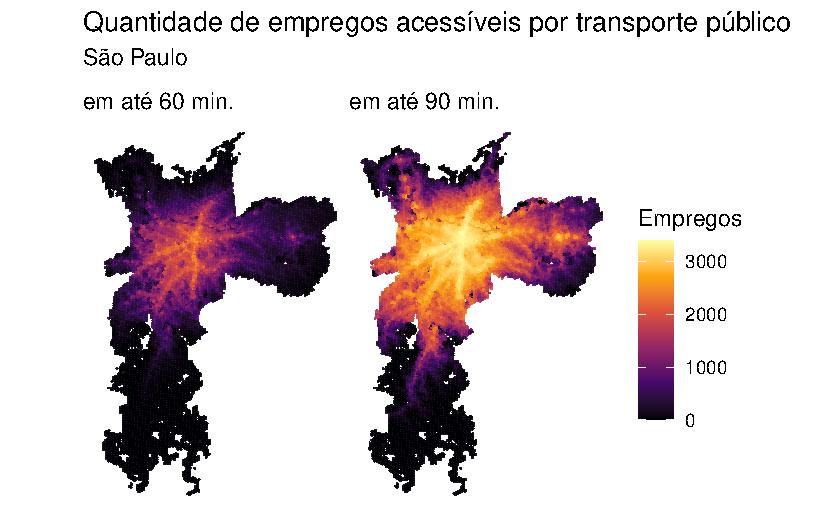
\includegraphics{./5_acessibilidade_files/figure-pdf/map CMATT60 vs CMATT90-1.pdf}

}

\end{figure}

\hypertarget{desigualdades-de-acesso-a-oportunidades}{%
\section{Desigualdades de acesso a
oportunidades}\label{desigualdades-de-acesso-a-oportunidades}}

Existem diversas maneiras de se analisar quão desiguais são as condições
de acesso a oportunidades a partir dos dados do \texttt{aopdata}. Nós
apresentamos nesta subseção dois exemplos de como esse tipo de análise
pode ser realizada.

\textbf{Desigualdade no tempo de acesso \texttt{TMI}}

Neste primeiro exemplo, nós vamos comparar qual o tempo médio de viagem
até o hospital mais próximo para pessoas de diferentes níveis de renda.
Para isso, o código abaixo calcula o valor médio de \texttt{TMISA}
ponderada pela população em cada hexágono. Essa ponderação é necessária
porque o número de hexágonos pode variar muito entre hexágonos.

Antes disso, cabe observar que alguns hexágonos da cidade não conseguem
acessar nenhum hospital em até 2h de viagem. Em casos como esse, o valor
das variáveis \texttt{TMI\_\_} é infinito (\texttt{Inf}). Para lidar com
esses casos, nós substituímos abaixo todos valores \texttt{Inf} por 120
minutos.

\begin{Shaded}
\begin{Highlighting}[]
\CommentTok{\# copy data to new data.table}
\NormalTok{dt }\OtherTok{\textless{}{-}} \FunctionTok{copy}\NormalTok{(df\_pt)}
\FunctionTok{setDT}\NormalTok{(dt)}

\CommentTok{\# replace Inf travel time with 120}
\NormalTok{dt[, TMISA }\SpecialCharTok{:}\ErrorTok{=} \FunctionTok{fifelse}\NormalTok{(TMISA}\SpecialCharTok{==}\ConstantTok{Inf}\NormalTok{, }\DecValTok{120}\NormalTok{, TMISA)]}

\CommentTok{\# calculate avarage travel time by income}
\NormalTok{temp }\OtherTok{\textless{}{-}}\NormalTok{ dt[, .(}\AttributeTok{average =} \FunctionTok{weighted.mean}\NormalTok{(}\AttributeTok{x=}\NormalTok{TMISA, }\AttributeTok{w=}\NormalTok{P001, }\AttributeTok{na.rm=}\NormalTok{T)), by}\OtherTok{=}\NormalTok{R003]}
\NormalTok{temp }\OtherTok{\textless{}{-}} \FunctionTok{na.omit}\NormalTok{(temp)}

\FunctionTok{ggplot}\NormalTok{() }\SpecialCharTok{+} 
  \FunctionTok{geom\_col}\NormalTok{(}\AttributeTok{data=}\NormalTok{temp, }\FunctionTok{aes}\NormalTok{(}\AttributeTok{y=}\NormalTok{average, }\AttributeTok{x=}\FunctionTok{factor}\NormalTok{(R003)), }\AttributeTok{fill=}\StringTok{\textquotesingle{}\#2c9e9e\textquotesingle{}}\NormalTok{, }\AttributeTok{color=}\ConstantTok{NA}\NormalTok{) }\SpecialCharTok{+}
  \FunctionTok{scale\_x\_discrete}\NormalTok{(}\AttributeTok{labels=}\FunctionTok{c}\NormalTok{(}\StringTok{"D1}\SpecialCharTok{\textbackslash{}n}\StringTok{+Pobres"}\NormalTok{, }\FunctionTok{paste0}\NormalTok{(}\StringTok{\textquotesingle{}D\textquotesingle{}}\NormalTok{, }\DecValTok{2}\SpecialCharTok{:}\DecValTok{9}\NormalTok{), }\StringTok{"D10}\SpecialCharTok{\textbackslash{}n}\StringTok{+Ricos"}\NormalTok{)) }\SpecialCharTok{+}
  \FunctionTok{labs}\NormalTok{(}\AttributeTok{title =} \StringTok{\textquotesingle{}Média de tempo de viagem até o hospital mais proximo\textquotesingle{}}\NormalTok{,}
       \AttributeTok{subtitle =} \StringTok{\textquotesingle{}por transporte público em São Paulo\textquotesingle{}}\NormalTok{,}
       \AttributeTok{x=}\StringTok{\textquotesingle{}Decil de renda\textquotesingle{}}\NormalTok{, }\AttributeTok{y=}\StringTok{\textquotesingle{}Tempo de viagem}\SpecialCharTok{\textbackslash{}n}\StringTok{em min.\textquotesingle{}}\NormalTok{) }\SpecialCharTok{+}
  \FunctionTok{theme\_minimal}\NormalTok{()}
\end{Highlighting}
\end{Shaded}

\begin{figure}[H]

{\centering 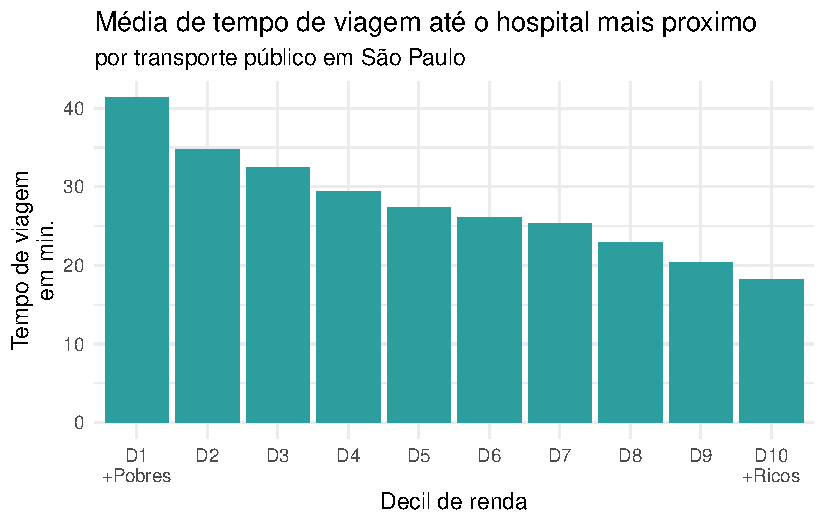
\includegraphics{./5_acessibilidade_files/figure-pdf/inequality TMISA-1.pdf}

}

\end{figure}

\textbf{Desigualdade do número de oportunidades acessíveis
\texttt{CAMA}}

Outra maneira de examinar a desigualdade de acesso a oportunidades é
comparar a quantidade de oportunidades acessíveis por diferentes grupos
populacionais considerando-se um mesmo modo de transporte e tempo de
viagem. Nesse caso, nós analisamos o Indicador de acessibilidade
cumulativo ativo (\texttt{CMA}).

Neste exemplo abaixo, nós utilizamos \emph{box plots} para comparar a
quantidade de empregos acessíveis por transporte público em até 30
minutos de viagem.

\begin{Shaded}
\begin{Highlighting}[]
\FunctionTok{ggplot}\NormalTok{() }\SpecialCharTok{+}
  \FunctionTok{geom\_boxplot}\NormalTok{(}\AttributeTok{data=}\FunctionTok{subset}\NormalTok{(dt, }\SpecialCharTok{!}\FunctionTok{is.na}\NormalTok{(R003)),}
               \FunctionTok{aes}\NormalTok{(}\AttributeTok{x =} \FunctionTok{factor}\NormalTok{(R003), }\AttributeTok{y=}\NormalTok{CMATT60}\SpecialCharTok{/}\DecValTok{1000}\NormalTok{, }\AttributeTok{color=}\FunctionTok{factor}\NormalTok{(R003))) }\SpecialCharTok{+}
  \FunctionTok{scale\_color\_brewer}\NormalTok{(}\AttributeTok{palette =} \StringTok{\textquotesingle{}RdBu\textquotesingle{}}\NormalTok{) }\SpecialCharTok{+}
  \FunctionTok{labs}\NormalTok{(}\AttributeTok{title=}\StringTok{\textquotesingle{}Distribução do número de empregos acessíveis em até 30 min.\textquotesingle{}}\NormalTok{, }\AttributeTok{color=}\StringTok{"Decil}\SpecialCharTok{\textbackslash{}n}\StringTok{de renda"}\NormalTok{,}
       \AttributeTok{subtitle=}\StringTok{\textquotesingle{}por transporte público, São Paulo\textquotesingle{}}\NormalTok{,}
       \AttributeTok{x=}\StringTok{\textquotesingle{}Decil de renda\textquotesingle{}}\NormalTok{, }\AttributeTok{y=}\StringTok{"N. de empregos acessíveis}\SpecialCharTok{\textbackslash{}n}\StringTok{(em milhares)"}\NormalTok{) }\SpecialCharTok{+}
  \FunctionTok{scale\_x\_discrete}\NormalTok{(}\AttributeTok{labels=}\FunctionTok{c}\NormalTok{(}\StringTok{"D1}\SpecialCharTok{\textbackslash{}n}\StringTok{+Pobres"}\NormalTok{, }\FunctionTok{paste0}\NormalTok{(}\StringTok{\textquotesingle{}D\textquotesingle{}}\NormalTok{, }\DecValTok{2}\SpecialCharTok{:}\DecValTok{9}\NormalTok{), }\StringTok{"D10}\SpecialCharTok{\textbackslash{}n}\StringTok{+Ricos"}\NormalTok{)) }\SpecialCharTok{+}
  \FunctionTok{theme\_minimal}\NormalTok{()}
\end{Highlighting}
\end{Shaded}

\begin{figure}[H]

{\centering 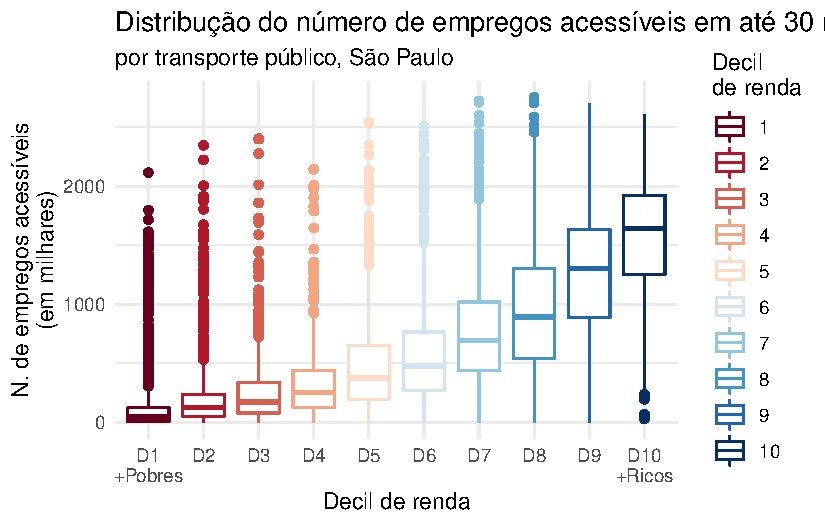
\includegraphics{./5_acessibilidade_files/figure-pdf/fig inequality CMATT30-1.pdf}

}

\end{figure}

\part{PARTE 3: Dados de transporte público}

Dados de transporte público são peças fundamentais no planejamento de
transportes em geral, e em análises de acessibilidade em particular.
Para serem usados de forma que se tenha segurança no resultado das
análises, esses dados precisam ser confiáveis e de simples inspeção e
interpretação.

Tentando satisfazer esses critérios, cada vez mais agências de
transporte público, tomadores de decisão e pesquisadores têm buscado
utilizar dados estruturados conforme especificações abertas e
colaborativas - ou seja, cujo formato seja decidido por uma comunidade
de atores interessados, incluindo partes que produzem esses dados
(agências de transporte público, por exemplo) e que os consomem
(pesquisadores, desenvolvedores de ferramentas de planejamento, etc.), e
não apenas por um único ator que dita, muitas vezes de forma pouco
transparente, os padrões a serem utilizados. Embora uma especificação
aberta não necessariamente resolva o problema da qualidade e da
confiabilidade dos dados por ela descritos, quando esta é amplamente
utilizada aumenta-se a confiabilidade da especificação em si. Além do
mais, cresce também a capacidade de inspeção dos dados e de sua
interpretação, visto que múltiplos atores detêm o conhecimento
necessário para tal.

A especificação de dados aberta e colaborativa mais amplamente utilizada
no contexto do planejamento de transporte público é o formato GTFS,
sigla para \emph{General Transit Feed Specification} (Especificação
Geral de Redes de Transporte Público, em tradução livre). Seus usos
abrangem tanto o planejamento quanto a operação de sistemas de
transporte público. Nesta seção nós iremos aprender o que são os dados
GTFS, como eles são estruturados e como utilizá-los, produzi-los e
modificá-los.

\hypertarget{dados-gtfs}{%
\chapter{Dados GTFS}\label{dados-gtfs}}

O formato GTFS, como comentado na introdução desta seção, é uma
especificação aberta e colaborativa que visa descrever os principais
componentes de uma rede de transporte público. Atualmente, dados GTFS
podem ser divididos em duas grandes categorias:

\begin{itemize}
\tightlist
\item
  GTFS Schedule, ou GTFS Static, que contém o cronograma estático de
  linhas de transporte público e informações espaciais sobre o
  itinerário de cada linha e suas paradas;
\item
  GTFS Realtime, que contém informações de localização de veículos em
  tempo real e alertas de possíveis atrasos, de mudanças de percurso e
  de eventos que possam interferir no cronograma planejado.
\end{itemize}

Ao longo desta seção, nós focaremos no \textbf{GTFS Schedule}. Clique
\href{https://gtfs.org/realtime/}{aqui} para mais informações sobre o
GTFS Realtime.

Por ser uma especificação aberta e colaborativa, o formato GTFS tenta
abarcar em sua definição um grande número de usos distintos que agências
de transporte e desenvolvedores de ferramentas possam dar a ele. No
entanto, agências e \emph{softwares} podem ainda assim depender de
informações que não constem na especificação oficial. Surgem, dessa
forma, \href{https://gtfs.org/extensions/}{extensões} da especificação.
Algumas dessas extensões podem eventualmente se tornar parte da
especificação oficial, caso isto seja aceito pela comunidade de usuários
do GTFS, enquanto a especificação de outras é continuamente desenvolvida
paralelamente à oficial. Nesta seção nós focaremos em um subconjunto de
informações presentes no formato GTFS Schedule ``puro'', e, portanto,
não cobriremos suas extensões.

\hypertarget{estrutura-dos-arquivos-de-gtfs}{%
\section{Estrutura dos arquivos de
GTFS}\label{estrutura-dos-arquivos-de-gtfs}}

\hypertarget{agency.txt}{%
\subsection{agency.txt}\label{agency.txt}}

A Table~\ref{tbl-agency} \ldots{}

\begin{verbatim}
agency_id,agency_name,agency_url,agency_timezone,agency_lang
1,SPTRANS,http://www.sptrans.com.br/?versao=011019,America/Sao_Paulo,pt 
\end{verbatim}

\hypertarget{tbl-agency}{}
\begin{longtable}[]{@{}
  >{\raggedright\arraybackslash}p{(\columnwidth - 8\tabcolsep) * \real{0.1075}}
  >{\raggedright\arraybackslash}p{(\columnwidth - 8\tabcolsep) * \real{0.1290}}
  >{\raggedright\arraybackslash}p{(\columnwidth - 8\tabcolsep) * \real{0.4409}}
  >{\raggedright\arraybackslash}p{(\columnwidth - 8\tabcolsep) * \real{0.1935}}
  >{\raggedright\arraybackslash}p{(\columnwidth - 8\tabcolsep) * \real{0.1290}}@{}}
\caption{\label{tbl-agency}Exemplo de tabela
\emph{agency}}\tabularnewline
\toprule()
\begin{minipage}[b]{\linewidth}\raggedright
agency\_id
\end{minipage} & \begin{minipage}[b]{\linewidth}\raggedright
agency\_name
\end{minipage} & \begin{minipage}[b]{\linewidth}\raggedright
agency\_url
\end{minipage} & \begin{minipage}[b]{\linewidth}\raggedright
agency\_timezone
\end{minipage} & \begin{minipage}[b]{\linewidth}\raggedright
agency\_lang
\end{minipage} \\
\midrule()
\endfirsthead
\toprule()
\begin{minipage}[b]{\linewidth}\raggedright
agency\_id
\end{minipage} & \begin{minipage}[b]{\linewidth}\raggedright
agency\_name
\end{minipage} & \begin{minipage}[b]{\linewidth}\raggedright
agency\_url
\end{minipage} & \begin{minipage}[b]{\linewidth}\raggedright
agency\_timezone
\end{minipage} & \begin{minipage}[b]{\linewidth}\raggedright
agency\_lang
\end{minipage} \\
\midrule()
\endhead
1 & SPTRANS & http://www.sptrans.com.br/?versao=011019 &
America/Sao\_Paulo & pt \\
\bottomrule()
\end{longtable}

\hypertarget{tbl-stops}{}
\begin{longtable}[]{@{}
  >{\raggedright\arraybackslash}p{(\columnwidth - 8\tabcolsep) * \real{0.0630}}
  >{\raggedright\arraybackslash}p{(\columnwidth - 8\tabcolsep) * \real{0.1654}}
  >{\raggedright\arraybackslash}p{(\columnwidth - 8\tabcolsep) * \real{0.6142}}
  >{\raggedleft\arraybackslash}p{(\columnwidth - 8\tabcolsep) * \real{0.0787}}
  >{\raggedleft\arraybackslash}p{(\columnwidth - 8\tabcolsep) * \real{0.0787}}@{}}
\caption{\label{tbl-stops}Exemplo de tabela \emph{stops}}\tabularnewline
\toprule()
\begin{minipage}[b]{\linewidth}\raggedright
stop\_id
\end{minipage} & \begin{minipage}[b]{\linewidth}\raggedright
stop\_name
\end{minipage} & \begin{minipage}[b]{\linewidth}\raggedright
stop\_desc
\end{minipage} & \begin{minipage}[b]{\linewidth}\raggedleft
stop\_lat
\end{minipage} & \begin{minipage}[b]{\linewidth}\raggedleft
stop\_lon
\end{minipage} \\
\midrule()
\endfirsthead
\toprule()
\begin{minipage}[b]{\linewidth}\raggedright
stop\_id
\end{minipage} & \begin{minipage}[b]{\linewidth}\raggedright
stop\_name
\end{minipage} & \begin{minipage}[b]{\linewidth}\raggedright
stop\_desc
\end{minipage} & \begin{minipage}[b]{\linewidth}\raggedleft
stop\_lat
\end{minipage} & \begin{minipage}[b]{\linewidth}\raggedleft
stop\_lon
\end{minipage} \\
\midrule()
\endhead
706325 & Parada 14 Bis B/C & Viad. Dr.~Plínio De Queiroz, 901 &
-23.55593 & -46.65011 \\
810602 & R. Sta. Rita, 56 & Ref.: R. Bresser / R. João Boemer &
-23.53337 & -46.61229 \\
910776 & Av. Do Estado, 5854 & Ref.: Rua Dona Ana Néri & -23.55896 &
-46.61520 \\
1010092 & Parada Caetano Pinto & Av. Rangel Pestana, 1249 Ref.: Rua
Caetano Pinto/rua Prof.~Batista De Andrade & -23.54615 & -46.62218 \\
1010093 & Parada Piratininga & Av. Rangel Pestana, 1479 Ref.: Rua
Monsenhor Andrade & -23.54509 & -46.62006 \\
1010099 & R. Xavantes, 612 & Ref.: Rua Joli & -23.53545 & -46.61368 \\
\bottomrule()
\end{longtable}

\hypertarget{tbl-routes}{}
\begin{longtable}[]{@{}
  >{\raggedright\arraybackslash}p{(\columnwidth - 12\tabcolsep) * \real{0.0857}}
  >{\raggedright\arraybackslash}p{(\columnwidth - 12\tabcolsep) * \real{0.0952}}
  >{\raggedright\arraybackslash}p{(\columnwidth - 12\tabcolsep) * \real{0.1619}}
  >{\raggedright\arraybackslash}p{(\columnwidth - 12\tabcolsep) * \real{0.2762}}
  >{\raggedleft\arraybackslash}p{(\columnwidth - 12\tabcolsep) * \real{0.1048}}
  >{\raggedright\arraybackslash}p{(\columnwidth - 12\tabcolsep) * \real{0.1143}}
  >{\raggedright\arraybackslash}p{(\columnwidth - 12\tabcolsep) * \real{0.1619}}@{}}
\caption{\label{tbl-routes}Exemplo de tabela
\emph{routes}}\tabularnewline
\toprule()
\begin{minipage}[b]{\linewidth}\raggedright
route\_id
\end{minipage} & \begin{minipage}[b]{\linewidth}\raggedright
agency\_id
\end{minipage} & \begin{minipage}[b]{\linewidth}\raggedright
route\_short\_name
\end{minipage} & \begin{minipage}[b]{\linewidth}\raggedright
route\_long\_name
\end{minipage} & \begin{minipage}[b]{\linewidth}\raggedleft
route\_type
\end{minipage} & \begin{minipage}[b]{\linewidth}\raggedright
route\_color
\end{minipage} & \begin{minipage}[b]{\linewidth}\raggedright
route\_text\_color
\end{minipage} \\
\midrule()
\endfirsthead
\toprule()
\begin{minipage}[b]{\linewidth}\raggedright
route\_id
\end{minipage} & \begin{minipage}[b]{\linewidth}\raggedright
agency\_id
\end{minipage} & \begin{minipage}[b]{\linewidth}\raggedright
route\_short\_name
\end{minipage} & \begin{minipage}[b]{\linewidth}\raggedright
route\_long\_name
\end{minipage} & \begin{minipage}[b]{\linewidth}\raggedleft
route\_type
\end{minipage} & \begin{minipage}[b]{\linewidth}\raggedright
route\_color
\end{minipage} & \begin{minipage}[b]{\linewidth}\raggedright
route\_text\_color
\end{minipage} \\
\midrule()
\endhead
CPTM L07 & 1 & CPTM L07 & JUNDIAI - LUZ & 2 & CA016B & \\
CPTM L08 & 1 & CPTM L08 & AMADOR BUENO - JULIO PRESTES & 2 & 97A098 & \\
CPTM L09 & 1 & CPTM L09 & GRAJAU - OSASCO & 2 & 01A9A7 & \\
CPTM L10 & 1 & CPTM L10 & RIO GRANDE DA SERRA - BRÁS & 2 & 049FC3 & \\
CPTM L11 & 1 & CPTM L11 & ESTUDANTES - LUZ & 2 & F68368 & \\
CPTM L12 & 1 & CPTM L12 & CALMON VIANA - BRAS & 2 & 133C8D & FFFFFF \\
\bottomrule()
\end{longtable}

\hypertarget{tbl-trips}{}
\begin{longtable}[]{@{}
  >{\raggedright\arraybackslash}p{(\columnwidth - 10\tabcolsep) * \real{0.1343}}
  >{\raggedright\arraybackslash}p{(\columnwidth - 10\tabcolsep) * \real{0.1642}}
  >{\raggedright\arraybackslash}p{(\columnwidth - 10\tabcolsep) * \real{0.1642}}
  >{\raggedright\arraybackslash}p{(\columnwidth - 10\tabcolsep) * \real{0.2090}}
  >{\raggedleft\arraybackslash}p{(\columnwidth - 10\tabcolsep) * \real{0.1940}}
  >{\raggedright\arraybackslash}p{(\columnwidth - 10\tabcolsep) * \real{0.1343}}@{}}
\caption{\label{tbl-trips}Exemplo de tabela \emph{trips}}\tabularnewline
\toprule()
\begin{minipage}[b]{\linewidth}\raggedright
route\_id
\end{minipage} & \begin{minipage}[b]{\linewidth}\raggedright
service\_id
\end{minipage} & \begin{minipage}[b]{\linewidth}\raggedright
trip\_id
\end{minipage} & \begin{minipage}[b]{\linewidth}\raggedright
trip\_headsign
\end{minipage} & \begin{minipage}[b]{\linewidth}\raggedleft
direction\_id
\end{minipage} & \begin{minipage}[b]{\linewidth}\raggedright
shape\_id
\end{minipage} \\
\midrule()
\endfirsthead
\toprule()
\begin{minipage}[b]{\linewidth}\raggedright
route\_id
\end{minipage} & \begin{minipage}[b]{\linewidth}\raggedright
service\_id
\end{minipage} & \begin{minipage}[b]{\linewidth}\raggedright
trip\_id
\end{minipage} & \begin{minipage}[b]{\linewidth}\raggedright
trip\_headsign
\end{minipage} & \begin{minipage}[b]{\linewidth}\raggedleft
direction\_id
\end{minipage} & \begin{minipage}[b]{\linewidth}\raggedright
shape\_id
\end{minipage} \\
\midrule()
\endhead
CPTM L07 & USD & CPTM L07-0 & JUNDIAI & 0 & 17846 \\
CPTM L07 & USD & CPTM L07-1 & LUZ & 1 & 17847 \\
CPTM L08 & USD & CPTM L08-0 & AMADOR BUENO & 0 & 17848 \\
CPTM L08 & USD & CPTM L08-1 & JULIO PRESTES & 1 & 17849 \\
CPTM L09 & USD & CPTM L09-0 & GRAJAU & 0 & 17850 \\
CPTM L09 & USD & CPTM L09-1 & OSASCO & 1 & 17851 \\
\bottomrule()
\end{longtable}

\hypertarget{tbl-calendar}{}
\begin{longtable}[]{@{}
  >{\raggedright\arraybackslash}p{(\columnwidth - 18\tabcolsep) * \real{0.1222}}
  >{\raggedleft\arraybackslash}p{(\columnwidth - 18\tabcolsep) * \real{0.0778}}
  >{\raggedleft\arraybackslash}p{(\columnwidth - 18\tabcolsep) * \real{0.0889}}
  >{\raggedleft\arraybackslash}p{(\columnwidth - 18\tabcolsep) * \real{0.1111}}
  >{\raggedleft\arraybackslash}p{(\columnwidth - 18\tabcolsep) * \real{0.1000}}
  >{\raggedleft\arraybackslash}p{(\columnwidth - 18\tabcolsep) * \real{0.0778}}
  >{\raggedleft\arraybackslash}p{(\columnwidth - 18\tabcolsep) * \real{0.1000}}
  >{\raggedleft\arraybackslash}p{(\columnwidth - 18\tabcolsep) * \real{0.0778}}
  >{\raggedright\arraybackslash}p{(\columnwidth - 18\tabcolsep) * \real{0.1222}}
  >{\raggedright\arraybackslash}p{(\columnwidth - 18\tabcolsep) * \real{0.1222}}@{}}
\caption{\label{tbl-calendar}Exemplo de tabela
\emph{calendar}}\tabularnewline
\toprule()
\begin{minipage}[b]{\linewidth}\raggedright
service\_id
\end{minipage} & \begin{minipage}[b]{\linewidth}\raggedleft
monday
\end{minipage} & \begin{minipage}[b]{\linewidth}\raggedleft
tuesday
\end{minipage} & \begin{minipage}[b]{\linewidth}\raggedleft
wednesday
\end{minipage} & \begin{minipage}[b]{\linewidth}\raggedleft
thursday
\end{minipage} & \begin{minipage}[b]{\linewidth}\raggedleft
friday
\end{minipage} & \begin{minipage}[b]{\linewidth}\raggedleft
saturday
\end{minipage} & \begin{minipage}[b]{\linewidth}\raggedleft
sunday
\end{minipage} & \begin{minipage}[b]{\linewidth}\raggedright
start\_date
\end{minipage} & \begin{minipage}[b]{\linewidth}\raggedright
end\_date
\end{minipage} \\
\midrule()
\endfirsthead
\toprule()
\begin{minipage}[b]{\linewidth}\raggedright
service\_id
\end{minipage} & \begin{minipage}[b]{\linewidth}\raggedleft
monday
\end{minipage} & \begin{minipage}[b]{\linewidth}\raggedleft
tuesday
\end{minipage} & \begin{minipage}[b]{\linewidth}\raggedleft
wednesday
\end{minipage} & \begin{minipage}[b]{\linewidth}\raggedleft
thursday
\end{minipage} & \begin{minipage}[b]{\linewidth}\raggedleft
friday
\end{minipage} & \begin{minipage}[b]{\linewidth}\raggedleft
saturday
\end{minipage} & \begin{minipage}[b]{\linewidth}\raggedleft
sunday
\end{minipage} & \begin{minipage}[b]{\linewidth}\raggedright
start\_date
\end{minipage} & \begin{minipage}[b]{\linewidth}\raggedright
end\_date
\end{minipage} \\
\midrule()
\endhead
USD & 1 & 1 & 1 & 1 & 1 & 1 & 1 & 2008-01-01 & 2020-05-01 \\
U\_\_ & 1 & 1 & 1 & 1 & 1 & 0 & 0 & 2008-01-01 & 2020-05-01 \\
US\_ & 1 & 1 & 1 & 1 & 1 & 1 & 0 & 2008-01-01 & 2020-05-01 \\
\_SD & 0 & 0 & 0 & 0 & 0 & 1 & 1 & 2008-01-01 & 2020-05-01 \\
\_\_D & 0 & 0 & 0 & 0 & 0 & 0 & 1 & 2008-01-01 & 2020-05-01 \\
\emph{S} & 0 & 0 & 0 & 0 & 0 & 1 & 0 & 2008-01-01 & 2020-05-01 \\
\bottomrule()
\end{longtable}

\hypertarget{tbl-shapes}{}
\begin{longtable}[]{@{}
  >{\raggedright\arraybackslash}p{(\columnwidth - 8\tabcolsep) * \real{0.1233}}
  >{\raggedleft\arraybackslash}p{(\columnwidth - 8\tabcolsep) * \real{0.1781}}
  >{\raggedleft\arraybackslash}p{(\columnwidth - 8\tabcolsep) * \real{0.1781}}
  >{\raggedleft\arraybackslash}p{(\columnwidth - 8\tabcolsep) * \real{0.2466}}
  >{\raggedleft\arraybackslash}p{(\columnwidth - 8\tabcolsep) * \real{0.2740}}@{}}
\caption{\label{tbl-shapes}Exemplo de tabela
\emph{shapes}}\tabularnewline
\toprule()
\begin{minipage}[b]{\linewidth}\raggedright
shape\_id
\end{minipage} & \begin{minipage}[b]{\linewidth}\raggedleft
shape\_pt\_lat
\end{minipage} & \begin{minipage}[b]{\linewidth}\raggedleft
shape\_pt\_lon
\end{minipage} & \begin{minipage}[b]{\linewidth}\raggedleft
shape\_pt\_sequence
\end{minipage} & \begin{minipage}[b]{\linewidth}\raggedleft
shape\_dist\_traveled
\end{minipage} \\
\midrule()
\endfirsthead
\toprule()
\begin{minipage}[b]{\linewidth}\raggedright
shape\_id
\end{minipage} & \begin{minipage}[b]{\linewidth}\raggedleft
shape\_pt\_lat
\end{minipage} & \begin{minipage}[b]{\linewidth}\raggedleft
shape\_pt\_lon
\end{minipage} & \begin{minipage}[b]{\linewidth}\raggedleft
shape\_pt\_sequence
\end{minipage} & \begin{minipage}[b]{\linewidth}\raggedleft
shape\_dist\_traveled
\end{minipage} \\
\midrule()
\endhead
17846 & -23.53517 & -46.63535 & 1 & 13.56768 \\
17846 & -23.53513 & -46.63548 & 2 & 95.99193 \\
17846 & -23.53494 & -46.63626 & 3 & 185.05103 \\
17846 & -23.53473 & -46.63710 & 4 & 211.43776 \\
17846 & -23.53466 & -46.63735 & 5 & 356.31088 \\
17846 & -23.53416 & -46.63866 & 6 & 483.96616 \\
\bottomrule()
\end{longtable}

\hypertarget{tbl-stop_times}{}
\begin{longtable}[]{@{}llllr@{}}
\caption{\label{tbl-stop_times}Exemplo de tabela
\emph{stop\_times}}\tabularnewline
\toprule()
trip\_id & arrival\_time & departure\_time & stop\_id &
stop\_sequence \\
\midrule()
\endfirsthead
\toprule()
trip\_id & arrival\_time & departure\_time & stop\_id &
stop\_sequence \\
\midrule()
\endhead
CPTM L07-0 & 04:00:00 & 04:00:00 & 18940 & 1 \\
CPTM L07-0 & 04:08:00 & 04:08:00 & 18920 & 2 \\
CPTM L07-0 & 04:16:00 & 04:16:00 & 18919 & 3 \\
CPTM L07-0 & 04:24:00 & 04:24:00 & 18917 & 4 \\
CPTM L07-0 & 04:32:00 & 04:32:00 & 18916 & 5 \\
CPTM L07-0 & 04:40:00 & 04:40:00 & 18965 & 6 \\
\bottomrule()
\end{longtable}

\hypertarget{tbl-frequencies}{}
\begin{longtable}[]{@{}lllr@{}}
\caption{\label{tbl-frequencies}Exemplo de tabela
\emph{frequencies}}\tabularnewline
\toprule()
trip\_id & start\_time & end\_time & headway\_secs \\
\midrule()
\endfirsthead
\toprule()
trip\_id & start\_time & end\_time & headway\_secs \\
\midrule()
\endhead
CPTM L07-0 & 04:00:00 & 04:59:00 & 720 \\
CPTM L07-0 & 05:00:00 & 05:59:00 & 360 \\
CPTM L07-0 & 06:00:00 & 06:59:00 & 360 \\
CPTM L07-0 & 07:00:00 & 07:59:00 & 360 \\
CPTM L07-0 & 08:00:00 & 08:59:00 & 360 \\
CPTM L07-0 & 09:00:00 & 09:59:00 & 480 \\
\bottomrule()
\end{longtable}

\hypertarget{onde-encontrar-gtfs-de-cidades-brasileiras}{%
\section{Onde encontrar GTFS de cidades
brasileiras}\label{onde-encontrar-gtfs-de-cidades-brasileiras}}

\hypertarget{como-extrair-anuxe1lises-buxe1sicas-de-um-gtfs-pacote-gtfstools}{%
\section{Como extrair análises básicas de um GTFS (pacote
gtfstools)}\label{como-extrair-anuxe1lises-buxe1sicas-de-um-gtfs-pacote-gtfstools}}

\hypertarget{cuxe1lculo-de-velocidade-das-linhas}{%
\section{Cálculo de velocidade das
linhas}\label{cuxe1lculo-de-velocidade-das-linhas}}

\hypertarget{cuxe1lculo-de-frequuxeancia-das-linhas}{%
\section{Cálculo de frequência das
linhas}\label{cuxe1lculo-de-frequuxeancia-das-linhas}}

\hypertarget{mapear-a-rede-de-transporte-puxfablico}{%
\section{Mapear a rede de transporte
público}\label{mapear-a-rede-de-transporte-puxfablico}}

\hypertarget{como-fazer-ediuxe7uxf5es-na-rede-de-transporte-puxfablico-pacote-gtfstools}{%
\section{Como fazer edições na rede de transporte público (pacote
gtfstools)}\label{como-fazer-ediuxe7uxf5es-na-rede-de-transporte-puxfablico-pacote-gtfstools}}

\part{PARTE 4: Calculando acessibilidade}

\hypertarget{calculando-acessibilidade-urbana-com-r5r}{%
\chapter{\texorpdfstring{Calculando acessibilidade urbana com
\texttt{r5r}}{Calculando acessibilidade urbana com r5r}}\label{calculando-acessibilidade-urbana-com-r5r}}

Objetivo: mostrar como calcular acessibilidade urbana usando o pacote
r5r

6.1 Função `accessibility\{r5r\}`, diferentes indicadores

6.2 Mapa de acessibilidade

\begin{Shaded}
\begin{Highlighting}[]
\DecValTok{1} \SpecialCharTok{+} \DecValTok{1}
\end{Highlighting}
\end{Shaded}

\begin{verbatim}
[1] 2
\end{verbatim}

\part{PARTE 5: Avaliação de impacto}

\hypertarget{comparando-a-acessibilidade-entre-dois-cenuxe1rios-de-transporte}{%
\chapter{Comparando a acessibilidade entre dois cenários de
transporte}\label{comparando-a-acessibilidade-entre-dois-cenuxe1rios-de-transporte}}

\textbf{Objetivo}: mostrar como avaliar o impacto de acessibilidade de
uma política que altera a frequência de algumas linhas de transporte

\hypertarget{alterar-frequuxeancia-de-gtfs}{%
\section{7.1 Alterar frequência de
GTFS}\label{alterar-frequuxeancia-de-gtfs}}

\hypertarget{calcular-acessibilidade-nos-cenuxe1rios-antes-e-depois}{%
\section{7.2 Calcular acessibilidade nos cenários antes e
depois}\label{calcular-acessibilidade-nos-cenuxe1rios-antes-e-depois}}

\hypertarget{mapa-do-impacto-de-acessibilidade}{%
\section{Mapa do impacto de
acessibilidade}\label{mapa-do-impacto-de-acessibilidade}}

\hypertarget{como-impacto-de-acessibilidade-se-distribui-entre-grupos-sociais}{%
\section{Como impacto de acessibilidade se distribui entre grupos
sociais}\label{como-impacto-de-acessibilidade-se-distribui-entre-grupos-sociais}}

\hypertarget{comparando-a-acessibilidade-entre-dois-cenuxe1rios-de-uso-do-solo}{%
\chapter{Comparando a acessibilidade entre dois cenários de uso do
solo}\label{comparando-a-acessibilidade-entre-dois-cenuxe1rios-de-uso-do-solo}}

\textbf{Objetivo}: mostrar como avaliar o impacto de acessibilidade de
uma política que (a) constrói nova escola, ou (b) aumenta densidade de
população em determinadas áreas da cidade

\hypertarget{simulauxe7uxe3o-de-aumentando-de-densidade-populacional}{%
\section{Simulação de aumentando de densidade
populacional}\label{simulauxe7uxe3o-de-aumentando-de-densidade-populacional}}

\hypertarget{calcular-acessibilidade-nos-cenuxe1rios-antes-e-depois-1}{%
\section{Calcular acessibilidade nos cenários antes e
depois}\label{calcular-acessibilidade-nos-cenuxe1rios-antes-e-depois-1}}

\hypertarget{mapa-do-impacto-de-acessibilidade-1}{%
\section{Mapa do impacto de
acessibilidade}\label{mapa-do-impacto-de-acessibilidade-1}}

\hypertarget{como-impacto-de-acessibilidade-se-distribui-entre-grupos-sociais-1}{%
\section{Como impacto de acessibilidade se distribui entre grupos
sociais}\label{como-impacto-de-acessibilidade-se-distribui-entre-grupos-sociais-1}}

\hypertarget{references}{%
\chapter*{References}\label{references}}
\addcontentsline{toc}{chapter}{References}

\hypertarget{refs}{}
\begin{CSLReferences}{1}{0}
\leavevmode\vadjust pre{\hypertarget{ref-banister2011trilogy}{}}%
Banister, David. 2011. {``The Trilogy of Distance, Speed and Time.''}
\emph{Journal of Transport Geography} 19 (4): 950--59.

\leavevmode\vadjust pre{\hypertarget{ref-bertolini2005sustainable}{}}%
Bertolini, Luca, Frank Le Clercq, and Loek Kapoen. 2005. {``Sustainable
Accessibility: A Conceptual Framework to Integrate Transport and Land
Use Plan-Making. Two Test-Applications in the Netherlands and a
Reflection on the Way Forward.''} \emph{Transport Policy} 12 (3):
207--20.

\leavevmode\vadjust pre{\hypertarget{ref-boisjoly2017get}{}}%
Boisjoly, Geneviève, and Ahmed M El-Geneidy. 2017. {``How to Get There?
A Critical Assessment of Accessibility Objectives and Indicators in
Metropolitan Transportation Plans.''} \emph{Transport Policy} 55:
38--50.

\leavevmode\vadjust pre{\hypertarget{ref-church2000transport}{}}%
Church, Andrew, Martin Frost, and Karen Sullivan. 2000. {``Transport and
Social Exclusion in London.''} \emph{Transport Policy} 7 (3): 195--205.

\leavevmode\vadjust pre{\hypertarget{ref-dijst2002opportunities}{}}%
Dijst, Martin, Tom de Jong, and Jan Ritsema van Eck. 2002.
{``Opportunities for Transport Mode Change: An Exploration of a
Disaggregated Approach.''} \emph{Environment and Planning B: Planning
and Design} 29 (3): 413--30. \url{https://doi.org/10.1068/b12811}.

\leavevmode\vadjust pre{\hypertarget{ref-dong2006moving}{}}%
Dong, Xiaojing, Moshe E Ben-Akiva, John L Bowman, and Joan L Walker.
2006. {``Moving from Trip-Based to Activity-Based Measures of
Accessibility.''} \emph{Transportation Research Part A: Policy and
Practice} 40 (2): 163--80.

\leavevmode\vadjust pre{\hypertarget{ref-farrington2005rural}{}}%
Farrington, John, and Conor Farrington. 2005. {``Rural Accessibility,
Social Inclusion and Social Justice: Towards Conceptualisation.''}
\emph{Journal of Transport Geography} 13 (1): 1--12.

\leavevmode\vadjust pre{\hypertarget{ref-geurs2004accessibility}{}}%
Geurs, Karst T, and Bert Van Wee. 2004. {``Accessibility Evaluation of
Land-Use and Transport Strategies: Review and Research Directions.''}
\emph{Journal of Transport Geography} 12 (2): 127--40.

\leavevmode\vadjust pre{\hypertarget{ref-kim2003space}{}}%
Kim, Hyun-Mi, and Mei-Po Kwan. 2003. {``Space-Time Accessibility
Measures: A Geocomputational Algorithm with a Focus on the Feasible
Opportunity Set and Possible Activity Duration.''} \emph{Journal of
Geographical Systems} 5 (1): 71--91.

\leavevmode\vadjust pre{\hypertarget{ref-levinson2020transport}{}}%
Levinson, David, and David King. 2020. {``Transport Access Manual: A
Guide for Measuring Connection Between People and Places.''}

\leavevmode\vadjust pre{\hypertarget{ref-lucas2016transport}{}}%
Lucas, Karen, Giulio Mattioli, Ersilia Verlinghieri, and Alvaro Guzman.
2016. {``Transport Poverty and Its Adverse Social Consequences.''} In
\emph{Proceedings of the Institution of Civil Engineers-Transport},
169:353--65. 6. Thomas Telford Ltd.

\leavevmode\vadjust pre{\hypertarget{ref-miller2018accessibility}{}}%
Miller, Eric J. 2018. {``Accessibility: Measurement and Application in
Transportation Planning.''} \emph{Transport Reviews} 38 (5): 551--55.

\leavevmode\vadjust pre{\hypertarget{ref-nassir2016utility}{}}%
Nassir, Neema, Mark Hickman, Ali Malekzadeh, and Elnaz Irannezhad. 2016.
{``A Utility-Based Travel Impedance Measure for Public Transit Network
Accessibility.''} \emph{Transportation Research Part A: Policy and
Practice} 88: 26--39.

\leavevmode\vadjust pre{\hypertarget{ref-neutens2012analysis}{}}%
Neutens, Tijs, Matthias Delafontaine, Darren M Scott, and Philippe De
Maeyer. 2012. {``An Analysis of Day-to-Day Variations in Individual
Space--Time Accessibility.''} \emph{Journal of Transport Geography} 23:
81--91.

\leavevmode\vadjust pre{\hypertarget{ref-neutens2010equity}{}}%
Neutens, Tijs, Tim Schwanen, Frank Witlox, and Philippe De Maeyer. 2010.
{``Equity of Urban Service Delivery: A Comparison of Different
Accessibility Measures.''} \emph{Environment and Planning A} 42 (7):
1613--35.

\leavevmode\vadjust pre{\hypertarget{ref-paez2012measuring}{}}%
Páez, Antonio, Darren M Scott, and Catherine Morency. 2012. {``Measuring
Accessibility: Positive and Normative Implementations of Various
Accessibility Indicators.''} \emph{Journal of Transport Geography} 25:
141--53.

\leavevmode\vadjust pre{\hypertarget{ref-papa2015accessibility}{}}%
Papa, Enrica, and Luca Bertolini. 2015. {``Accessibility and
Transit-Oriented Development in European Metropolitan Areas.''}
\emph{Journal of Transport Geography} 47: 70--83.

\leavevmode\vadjust pre{\hypertarget{ref-pereira2022acessibilidade}{}}%
Pereira, Rafael H. M., Carlos Kauê Vieira Braga, Daniel Herszenhut,
Marcus Saraiva, and Diego Bogado Tomasiello. 2022. {``Estimativas de
Acessibilidade a Empregos e Serviços Públicos via Transporte Ativo,
Público e Privado Nas 20 Maiores Cidades Do Brasil Em 2017, 2018,
2019.''} \emph{Texto Para Discuss{ã}o IPEA} preliminar.
\url{https://www.ipea.gov.br/portal/publicacao-item?id=11058/11345}.

\leavevmode\vadjust pre{\hypertarget{ref-pereira2022usosolo}{}}%
Pereira, Rafael H. M., Daniel Herszenhut, Carlos Kauê Vieira Braga, João
Bazzo, João Lucas Albuquerque Oliveira, João Parga, Marcus Saraiva, Luiz
Pedro Silva, Diego Bogado Tomasiello, and Lucas Warwar. 2022.
{``Distribuição Espacial de Características Sociodemográficas e
Localização de Empregos e Serviços Públicos Das Vinte Maiores Cidades Do
Brasil.''} \emph{Texto Para Discuss{ã}o IPEA} 2772.
\url{http://repositorio.ipea.gov.br/handle/11058/11225}.

\leavevmode\vadjust pre{\hypertarget{ref-pereira2017distributive}{}}%
Pereira, Rafael HM, Tim Schwanen, and David Banister. 2017.
{``Distributive Justice and Equity in Transportation.''} \emph{Transport
Reviews} 37 (2): 170--91.

\leavevmode\vadjust pre{\hypertarget{ref-van2022accessibility}{}}%
Wee, Bert van. 2022. {``Accessibility and Equity: A Conceptual Framework
and Research Agenda.''} \emph{Journal of Transport Geography} 104:
103421.

\end{CSLReferences}

\appendix
\addcontentsline{toc}{part}{Appendices}

\hypertarget{nouxe7uxf5es-buxe1sicas-de-r}{%
\chapter{Noções básicas de R}\label{nouxe7uxf5es-buxe1sicas-de-r}}

\hypertarget{objetos}{%
\section{Objetos}\label{objetos}}

\begin{Shaded}
\begin{Highlighting}[]
\NormalTok{a }\OtherTok{\textless{}{-}} \DecValTok{1}

\NormalTok{a }\SpecialCharTok{+} \DecValTok{1}
\end{Highlighting}
\end{Shaded}

\begin{verbatim}
[1] 2
\end{verbatim}

\begin{Shaded}
\begin{Highlighting}[]
\NormalTok{a }\OtherTok{\textless{}{-}} \FunctionTok{c}\NormalTok{(}\DecValTok{1}\NormalTok{,}\DecValTok{2}\NormalTok{,}\DecValTok{3}\NormalTok{)}

\NormalTok{a }\SpecialCharTok{+} \DecValTok{1}
\end{Highlighting}
\end{Shaded}

\begin{verbatim}
[1] 2 3 4
\end{verbatim}

Texto

\begin{Shaded}
\begin{Highlighting}[]
\NormalTok{a }\OtherTok{\textless{}{-}} \StringTok{"Bom dia"}

\FunctionTok{paste}\NormalTok{(a, }\StringTok{\textquotesingle{}Joana\textquotesingle{}}\NormalTok{)}
\end{Highlighting}
\end{Shaded}

\begin{verbatim}
[1] "Bom dia Joana"
\end{verbatim}

\hypertarget{data.frames}{%
\section{Data.frames}\label{data.frames}}

\hypertarget{como-importar-e-exportar-arquivos}{%
\section{Como importar e exportar
arquivos}\label{como-importar-e-exportar-arquivos}}

\hypertarget{funuxe7uxf5es}{%
\section{Funções}\label{funuxe7uxf5es}}

\hypertarget{visualizauxe7uxe3o-de-dados-com-ggplot2}{%
\section{\texorpdfstring{Visualização de dados com
\texttt{ggplot2}}{Visualização de dados com ggplot2}}\label{visualizauxe7uxe3o-de-dados-com-ggplot2}}

```



\end{document}
